% Optimal Liquidation under Execution Constraints
% Applied Mathematical Finance submission - Interact layout, APA reference style

\documentclass[]{interact}

\usepackage{epstopdf}
\usepackage[caption=false]{subfig}

\usepackage[longnamesfirst,sort]{natbib}
\bibpunct[, ]{(}{)}{;}{a}{,}{,}
\renewcommand\bibfont{\fontsize{10}{12}\selectfont}

% --- additional packages for math, figures, tables --------------------------
\usepackage{amsmath, amssymb, mathtools}
\usepackage{booktabs}
\usepackage{graphicx}
\usepackage{xcolor}
\usepackage{microtype}
\usepackage{hyperref}
\hypersetup{colorlinks=true, linkcolor=blue, citecolor=blue, urlcolor=blue}

% Theorem environments (interact.cls compatible)
\theoremstyle{plain}
\newtheorem{theorem}{Theorem}[section]
\newtheorem{lemma}[theorem]{Lemma}
\newtheorem{corollary}[theorem]{Corollary}
\newtheorem{proposition}[theorem]{Proposition}

\theoremstyle{definition}
\newtheorem{definition}[theorem]{Definition}
\newtheorem{assumption}[theorem]{Assumption}

\theoremstyle{remark}
\newtheorem{remark}{Remark}

% --- author macros ----------------------------------------------------------
\newcommand{\R}{\mathbb{R}}
\newcommand{\E}{\mathbb{E}}
\newcommand{\Prob}{\mathbb{P}}
\newcommand{\1}[1]{\mathbf{1}_{\{#1\}}}
\newcommand{\esssup}{\mathop{\mathrm{ess\,sup}}}
\newcommand{\argmax}{\mathop{\mathrm{arg\,max}}}
\newcommand{\ltil}{\widetilde{\lambda}}

\begin{document}

\articletype{RESEARCH ARTICLE}

\title{Sample Complexity of Calibration versus Model-Free Learning in Cartea--Jaimungal--Penalva Optimal Liquidation}

\author{
\name{Wendi Ouyang\textsuperscript{a}\thanks{CONTACT Wendi Ouyang. Email: 122010063@link.cuhk.edu.cn}}
\affil{\textsuperscript{a}School of Science and Engineering, Department of Statistics and Data Science, The Chinese University of Hong Kong, Shenzhen, Shenzhen, Guangdong, China}
}

\maketitle

\begin{abstract}
We construct a sample-complexity benchmark for optimal liquidation in the \citet{cjp2015} (CJP) Poisson-fill limit-order/market-order framework, comparing model-free reinforcement learning (RL) against a parametric model-based calibrator that estimates $(\kappa,\lambda)$ and plans by one finite-difference solve of the CJP quasi-variational inequality. In the CJP Chapter~8 scale ($Q_0=10$, $T=60$s), the plug-in MLE attains about $+0.194$ dollars per episode relative to TWAP---matching the FD-optimal premium to within Monte-Carlo error. By contrast, Double DQN saturates near $+0.129$ and a structure-aware hybrid PPO reaches about $+0.135$ after removing a depth-floor artefact, but clears inventory in only about $23\%$ of evaluation paths. We then add an institutional-scale stress test ($Q_0=100$, $T=600$s). In this larger regime, cash premium alone is statistically inconclusive: Hybrid PPO has the largest point estimate, but no learned-agent difference from Plug-in MLE survives Holm-corrected pairwise testing, and Plug-in MLE remains the only method combining FD-level value accuracy, high pre-terminal clearance, and negligible compute. We attribute these findings to three forces: (i) a reward-shaping identity (Theorem~\ref{thm:reward-shaping}) under which the expected return of any policy equals the reduced value function $h(t, q)$; (ii) a CIR-type stochastic intensity extension validated at $\lambda_0\in\{0.7\bar\lambda,\bar\lambda,1.3\bar\lambda\}$ for $\sigma_\lambda \in [0,0.1]$; and (iii) a parameter robustness analysis showing the FD-optimal policy degrades gracefully under factor-of-two microstructure misspecification once the terminal-impact face-lift is implemented correctly. The resulting message is not that calibration always maximises cash premium, but that, inside a correct low-dimensional CJP model class, stronger modelling assumptions buy orders-of-magnitude gains in sample efficiency, value accuracy, and completion stability.
\end{abstract}

\begin{keywords}
optimal execution; quasi-variational inequality; reinforcement learning;
Hamilton--Jacobi--Bellman; stochastic intensity; sample complexity;
limit order book; Cox--Ingersoll--Ross intensity
\end{keywords}


% ============================================================================
\section{Introduction}\label{sec:intro}
% ============================================================================

Institutional liquidation of large positions trades off price uncertainty against execution cost. The discrete-time formulation of \citet{bertsimaslo1998} and the continuous-time analogue of \citet{almgrenchriss2001} delivered closed-form deterministic schedules under linear impact; \citet{obizhaevawang2013} extended this line to a stochastic supply/demand process. The richer microstructure model of \citet{cjp2015} (henceforth CJP) embedded the same objective into a Poisson-fill limit-order book and obtained a tractable quasi-variational inequality (QVI) that delivers the agent's depth posting and market-order trigger jointly; related LOB-control and numerical-HJB treatments include \citet{bayraktarludkovski2014}, \citet{forsyth2011hjb}, and the book-length account of \citet{gueant2016marketliquidity}. Subsequent CJP-style extensions cover model uncertainty \citep{cartea2017uncertainty, cartea2018sigest} and Hawkes-type self-excitation \citep{alfonsi2016hawkes}. For the empirical microstructure background we refer to the comprehensive treatments of \citet{bouchaud2018trades} and \citet{contstoikovtalreja2010}. The CJP reduction via the ansatz $H(t,x,S,q) = x + qS + h(t,q)$ exposes a one-dimensional dynamic-programming problem in $h$ that admits closed-form solutions for small inventory and rapid numerical solution for general $q$ via standard impulse-control numerical methods \citep{pham2009stochastic, forsythvetzal2002}.

Reinforcement learning has emerged as a popular data-driven alternative when microstructure parameters are unknown or non-stationary. \citet{nevmyvaka2006rl} introduced Q-learning for execution scheduling; \citet{hendrickswilcox2014} added an RL layer to the \citet{almgrenchriss2001} schedule; \citet{linbeling2020} applied end-to-end PPO to execution; \citet{ninglinjaimungal2021} trained a Double DQN on a CJP-like environment with raw limit-order-book features and reported a $+6.5$-bps premium over TWAP. Recent surveys \citep{hambly2023rlfinance, charpentier2023rlecon} document the broader landscape of RL applications in quantitative finance. The promise of this line of work is that, by foregoing explicit microstructure modelling, RL controllers can adapt to environments where the CJP assumptions partially fail.

Our experiments suggest this promise should be qualified. In a CJP-faithful simulator at the CJP Chapter~8 scale, a Double DQN with $\sim 5\,000$ parameters saturates near a $+0.129$ dollar premium per $10$-share liquidation episode and is dominated by a two-parameter MLE that attains the FD-optimal premium of about $+0.194$ from a small observed-fill sample. Equivalently, the plug-in premium is about $1.9$ cents per share, or $6.5$ basis points at the baseline midprice $S_0=\$30$. The gap does not close with sample budget: at $n = 10^5$ environment transitions---two orders of magnitude beyond what is feasible on real high-frequency data within a calibration window---DDQN still trails the MLE. A structure-aware hybrid policy that hard-wires the CJP exponential ansatz $\hat\kappa^{-1}$ into the architecture closes part of the parameter-efficiency gap but not the premium gap at this scale, suggesting that the bottleneck is the model-free RL route rather than merely DDQN's implementation.

Because the CJP Chapter~8 benchmark uses a deliberately small inventory, we also report a scale stress test with $Q_0=100$ and $T=600$s. Since both inventory and horizon increase by the same factor, the baseline fill intensity $\lambda=50/60$ is kept fixed so that $\lambda T/Q_0$ is unchanged. The stress test changes the interpretation rather than simply amplifying the headline result: pure passive posting loses its apparent dominance once clearance is inspected, while some RL seed means tilt toward higher cash premium at the expense of value-function accuracy and completion. The plug-in calibrator remains the only method that both matches the FD solution and stays computationally negligible.

We make four contributions in support of this picture. First, we construct a reward shaping (Theorem~\ref{thm:reward-shaping}) under which the expected cumulative return of any policy equals the reduced value function $h(t, q)$. This shaping promotes the Monte-Carlo premium comparison used by prior work to a pointwise diagnostic $\|V_\pi(t,q) - h(t,q)\|_\infty$ measurable on the FD reference grid. Second, we empirically characterise the sample-efficiency frontier between a strong parametric model-based planner and model-free RL on the CJP Chapter~8 scale. An exact-Bernoulli MLE of $(\hat\kappa, \hat\lambda)$ combined with one backward FD pass at the fitted parameters achieves the FD-optimal premium at every sample budget from $10^2$ to $10^5$, while Tabular Q and DDQN remain below it. Third, we propose and evaluate a structure-aware hybrid policy class ($\delta_\theta = \hat\kappa^{-1} + g_\theta$, with $g_\theta$ a signed bounded residual MLP) trained via clipped Proximal Policy Optimization \citep{schulman2017ppo}. The Regime-II stress test shows why premium alone is not enough: the hybrid's mean raw premium can be higher within seed-level noise, but it remains inaccurate and incomplete relative to the FD-matching calibrator. Fourth, we extend the framework to a CIR-type stochastic fill intensity (Lemma~\ref{lem:cir-ansatz}), derive the reduced HJB, and solve it with an upwind backward-Euler scheme. We validate the $\sigma_\lambda \to 0$ limit explicitly on $\sigma_\lambda \in [0,0.1]$ at three intensity slices; the high-volatility regime is treated as a numerical extension rather than as a validation claim.

The remainder of the paper is structured as follows. Section~\ref{sec:model} fixes notation and the model. Section~\ref{sec:lo-only} reviews the LO-only benchmark of \citet{carteajaimungal2015}. Section~\ref{sec:lo-mo} treats LO+MO with the FD QVI. Section~\ref{sec:rl} sets up the four-agent benchmark and presents the structure-aware hybrid. Section~\ref{sec:cir} adds the CIR-intensity extension. Section~\ref{sec:robustness} reports parameter robustness and misspecification. Section~\ref{sec:baselines} extends the baseline panel. Section~\ref{sec:discussion} discusses implications and limitations; Section~\ref{sec:conclusion} concludes.

% ============================================================================
\section{Model and notation}\label{sec:model}
% ============================================================================

We follow the discrete-time LO/MO model of \citet[Chapter 8]{cjp2015} on a fixed horizon $T$. The agent's objective is to liquidate an initial inventory $Q_0$ shares by time $T$ while balancing the LO fill premium against running inventory variance and a forced-liquidation cost.
The baseline $Q_0=10$ is the small pedagogical inventory scale used in the CJP Chapter~8 numerical example; Section~\ref{sec:limitations} discusses the scaling limitation.
Unless otherwise stated, implementation premiums are reported in dollars per complete liquidation episode relative to TWAP. Dividing by $Q_0$ gives dollars per share.
For the scale stress test in Section~\ref{sec:regime-ii}, we use $Q_0=100$, $T=600$s, $S_0=30$, $\lambda=50/60$, $\kappa=100$, $\xi=0.005$, $\alpha=10^{-5}$, and $\phi=10^{-6}$. Keeping $\lambda$ fixed preserves the expected external-arrival density per share, $\lambda T/Q_0$, because $Q_0$ and $T$ are both scaled by $10$.

\subsection{Notation}\label{sec:notation}
Table~\ref{tab:notation} lists every symbol used in the paper.

\begin{table}[t]
\centering
\caption{Notation. All quantities are in seconds, dollars, and shares as appropriate.}
\label{tab:notation}
\begin{tabular}{@{}lll@{}}
\toprule
Symbol & Meaning & Default value \\
\midrule
$T$ & trading horizon & $60$ s \\
$Q_0$ & initial inventory & $10$ shares \\
$q$ & remaining inventory & $0,\dots,Q_0$ \\
$\delta$ & posted LO depth above the mid & $\ge 0$ \\
$S_t$ & midprice (arithmetic Brownian) & --- \\
$S_0$ & initial midprice & $30$ \$ \\
$\sigma$ & midprice volatility & $0.01$ \$/$\sqrt{\text{s}}$ \\
$\lambda$ & arrival rate of external MOs & $50/60$ s$^{-1}$ \\
$\kappa$ & depth-decay parameter & $100$ \$$^{-1}$ \\
$\xi$ & half-spread paid on agent MOs & $0.005$ \$ \\
$\alpha$ & quadratic terminal-impact coefficient & $10^{-3}$ \$/share$^2$ \\
$\phi$ & running inventory-penalty coefficient & $10^{-5}$ \$/share$^2$/s \\
$\ltil$ & effective rate $\lambda / e$ after optimising $\delta$ & --- \\
$h(t,q)$ & reduced value function from ansatz $H = x + qS + h$ & --- \\
$\omega(t,q)$ & exponential transform $e^{\kappa h}$ & --- \\
$\kappa_\lambda$ & CIR mean-reversion speed for $\lambda_t$ & $2.0$ \\
$\bar\lambda$ & CIR long-run mean & $50/60$ s$^{-1}$ \\
$\sigma_\lambda$ & CIR vol-of-vol & $0.1$ \\
\bottomrule
\end{tabular}
\end{table}

\begin{definition}[Admissible controls]\label{def:admissible}
Let $\mathbb{F}=(\mathcal{F}_t)_{0\le t\le T}$ be the natural filtration generated by the midprice Brownian motion, the external order-flow randomness, and the controlled counting processes. A control pair $(\delta,M)$ is admissible if $\delta$ is $\mathbb{F}$-predictable with $0\le\delta_t\le\delta_{\max}<\infty$, $M$ is a simple $\mathbb{F}$-adapted point process with unit jumps and $\mathbb{E}[M_T]<\infty$, and the induced inventory remains in $\{0,\ldots,Q_0\}$, so $M$ can jump only when $Q_{t^-}>0$. We denote this class by $\mathcal{A}$.
\end{definition}

\subsection{LO/MO dynamics}\label{sec:lomo-dynamics}
The midprice follows
\begin{equation}\label{eq:midprice}
dS_t = \sigma\, dW_t,
\end{equation}
with $S_0$ given. The driftless midprice is the CJP short-horizon assumption: over the $60$-second liquidation window, directional drift is treated as negligible relative to execution costs and volatility. The agent posts a single unit-size LO at depth $\delta_t \ge 0$ above the prevailing mid. External MOs arrive as a Poisson process of rate $\lambda$; conditional on an arrival, the agent's LO is hit with probability
\begin{equation}\label{eq:fillprob}
P(\delta) = e^{-\kappa \delta}.
\end{equation}
The agent may also fire a unit MO at any time, paying half the spread $\xi$ per share. Inventory evolves as
\begin{equation}\label{eq:invsde}
dQ^{\delta,M}_t = - dN^{\delta}_t - dM_t,
\end{equation}
where $N^\delta$ counts agent LO fills and $M$ counts agent MOs. Cash accumulates as
\begin{equation}\label{eq:cashsde}
dX^{\delta,M}_t = (S_{t-} + \delta_{t-})\, dN^\delta_t + (S_{t-} - \xi)\, dM_t.
\end{equation}
The agent's performance criterion is
\begin{equation}\label{eq:performance}
H(t,x,S,q) = \esssup_{(\delta, M)\in\mathcal{A}}\, \E\!\left[ X_T + Q_T (S_T - \alpha Q_T)
- \phi \!\int_t^T\! Q_s^2\, ds \,\Big|\, X_t = x,\, S_t = S,\, Q_t = q \right].
\end{equation}
The terminal expression marks any residual inventory to a block-liquidation value with quadratic impact; the agent can alternatively fire market orders immediately before maturity and pay the half-spread cost. This produces the face-lifted boundary used below, $h(T^-,q)=\max\{-\alpha q^2,-q\xi\}$. The $-\phi \int_t^T Q_s^2\, ds$ term penalises holding inventory during the trading interval; we use the predictable left-continuous inventory convention for the integrand, which is immaterial for finitely many jump times under Lebesgue integration.

\subsection{Structural decomposition}\label{sec:ansatz}
\begin{proposition}[Ansatz validity]\label{prop:ansatz}
Under \eqref{eq:midprice}--\eqref{eq:performance}, the value function admits the additive separation
\begin{equation}\label{eq:ansatz}
H(t,x,S,q) = x + q S + h(t,q),
\end{equation}
where $h$ depends only on $(t,q)$ and is bounded on $[0,T] \times \{0,\dots,Q_0\}$. In particular $h(t,0) = 0$ for all $t \le T$, $h(T,q)=-\alpha q^2$, and the pre-terminal face-lift is
$h(T^-, q) = \max\{-\alpha q^2, -q\xi\}$.
\end{proposition}
\begin{proof}[Proof sketch]
The midprice is a martingale, so $\E[q S_T - q S_t]= 0$ and the cash component $x$ adds linearly. The face-lift follows by comparing the terminal block liquidation value $-\alpha q^2$ with firing $q$ unit market orders immediately before $T$ at total half-spread cost $q\xi$, as in \citet[\S 8]{cjp2015}.
\end{proof}

Throughout we work with the reduced function $h(t,q)$, and we use the exponential transform
\begin{equation}\label{eq:omega}
\omega(t,q) = e^{\kappa h(t,q)}
\end{equation}
freely; the LO-only solution \eqref{eq:omega-poisson} below is expressed most cleanly in $\omega$.

% ============================================================================
\section{Benchmark: limit-orders only}\label{sec:lo-only}
% ============================================================================

This section uses the LO-only degeneracy $\xi=\phi=0$ as an analytical benchmark, not the LO+MO parameter regime used in Sections~\ref{sec:lo-mo}--\ref{sec:baselines}. When $\xi = \phi = 0$ the agent only ever posts LOs and the reduced HJB becomes the ODE system
\begin{equation}\label{eq:lo-hjb}
\partial_t h(t,q) + \sup_\delta \lambda e^{-\kappa \delta}\bigl[ \delta + h(t,q-1) - h(t,q)\bigr] = 0,
\quad h(t,0) = 0,
\end{equation}
with terminal $h(T,q) = -\alpha q^2$. In the LO-only regime ($\xi = \phi = 0$) the supremum is attained at the unique interior maximiser
\begin{equation}\label{eq:delta-star-lo}
\delta^*(t,q) = \kappa^{-1} + h(t,q) - h(t,q-1).
\end{equation}
In the LO+MO setting of Section~\ref{sec:lo-mo}, \eqref{eq:delta-star-lo} remains the continuation-operator inner argmax---i.e., the optimal depth conditional on \emph{not} firing an MO at the current step---and serves as the structural anchor for the hybrid policy of Section~\ref{sec:rl}. Substituting \eqref{eq:delta-star-lo} back into \eqref{eq:lo-hjb} gives the closed-form solution
\begin{equation}\label{eq:omega-poisson}
\omega(t,q) = \sum_{n=0}^{q} \frac{\ltil^n}{n!} e^{-\kappa\alpha (q-n)^2} (T-t)^n,
\qquad \ltil = \lambda / e,
\end{equation}
of \citet[\S 8.2]{cjp2015}. The optimal depth has two interpretable terms: a $\kappa^{-1}$ ``asymptote'' equal to the depth that maximises the per-fill premium $\delta e^{-\kappa \delta}$, and a log-likelihood-ratio correction $h(t,q) - h(t,q-1)$ that captures the marginal continuation value of holding one fewer share. The asymptote $\kappa^{-1}$ is the structural prior we exploit in the hybrid policy of Section~\ref{sec:rl}.

The LO-only formula is used only to motivate the depth asymptote and the CJP exponential transform. The full sample-complexity comparison appears in Section~\ref{sec:sample-complexity}, where the market-order action, half-spread cost, running inventory penalty, and face-lift boundary are all active.

% ============================================================================
\section{Mixed control: limit and market orders}\label{sec:lo-mo}
% ============================================================================

When $\xi > 0$ and $\phi > 0$ the agent has a non-trivial choice between waiting for an LO fill and crossing the spread with an MO. The reduced QVI of \citet{carteajaimungal2015} is
\begin{equation}\label{eq:qvi}
\begin{split}
\max\Bigl\{
&\partial_t h - \phi q^2 + \frac{\ltil}{\kappa}\, e^{-\kappa[h(t,q)-h(t,q-1)]}\, ;\\
&- \xi + h(t,q-1) - h(t,q) \Bigr\} = 0,
\end{split}
\end{equation}
with $h(t,0) = 0$ and the face-lifted terminal $h(T^-, q) = \max\{-\alpha q^2,-q\xi\}$. The two arguments of $\max$ correspond to continuation (post an LO) and intervention (fire an MO), respectively; the QVI is active where the intervention argument matches the continuation argument, defining the MO trigger boundary.

\begin{theorem}[QVI well-posedness]\label{thm:qvi}
Under Assumption $\xi, \alpha, \phi \ge 0$ and the running-cost integrability of \eqref{eq:performance}, the QVI \eqref{eq:qvi} admits a unique bounded solution $h:[0,T]\times\{0,\dots,Q_0\}\to\mathbb{R}$, continuous in $t$ and satisfying the stated boundary and face-lift terminal conditions. The associated optimal policy is feedback in $(t,q)$.
\end{theorem}
\begin{proof}[Proof reference]
The QVI \eqref{eq:qvi} is the dynamic-programming equation of a finite-state impulse-control problem with state $(t, q) \in [0,T] \times \{0, \dots, Q_0\}$, inventory-only impulse ($q \mapsto q - 1$ at cost $\xi$), and continuous control $\delta \in [0, \delta_{\max}]$. The finite-state standard result of \citet[\S 5.4]{pham2009stochastic} applies once the continuation operator is locally Lipschitz in the finite set of inventory coordinates. An independent a priori bound follows by comparison with immediate market-order liquidation and with the bounded terminal payoff: for all $q$, $-q\xi-\phi q^2T-\alpha q^2 \le h(t,q) \le \delta_{\max}q$. Hence $|\Delta_q h|$ is bounded by a constant depending only on $(Q_0,\xi,\alpha,\phi,T,\delta_{\max})$, and $\sup_\delta \lambda e^{-\kappa\delta}[\delta+\Delta_q h]$ is locally Lipschitz on the resulting compact range. The feedback structure of the optimal policy is standard for finite-state impulse problems; comparison-principle arguments such as \citet[Theorem 4.1]{bouchardtouzi2011} give the analogous uniqueness statement in continuous spatial domains.
\end{proof}

\subsection{Analytical solution for $q \in \{1,2\}$}\label{sec:q12-analytic}
For orientation, consider the spread-face-lift subcase in which the terminal branch is $h(T^-,q)=-q\xi$. This is the closed-form calculation in CJP and is useful for reading the free-boundary geometry, while the numerical experiments below use the full terminal condition $\max\{-\alpha q^2,-q\xi\}$. For $q = 1$ in the continuation regime $\phi \le \ltil e^{\kappa\xi} / \kappa$, integrating the QVI gives
\begin{equation}\label{eq:omega-q1}
\omega(t,1) = e^{-\kappa\xi} e^{-\kappa\phi(T-t)}
+ \frac{\ltil}{\kappa\phi}\bigl(1 - e^{-\kappa\phi(T-t)}\bigr).
\end{equation}
For the main-regime parameters, $\phi/(\ltil e^{\kappa\xi}/\kappa)\approx 2\times10^{-3}\ll 1$, so this continuation-regime condition is comfortably satisfied.
For $q = 2$ there is a critical time $\tau_2 \in (0, T]$ at which the MO trigger first activates; on $[0, \tau_2)$ the continuation ODE applies, and on $[\tau_2, T]$ the trigger is on and $\omega(t,2) = e^{-\kappa\xi} \omega(t,1)$. The critical time solves
\begin{equation}\label{eq:tau2}
\omega(\tau_2, 1) = \frac{\ltil e^{\kappa\xi}}{\ltil - 3\kappa\phi e^{-\kappa\xi}}.
\end{equation}

\subsection{Finite-difference scheme}\label{sec:fd}
For general $q$ we discretise time uniformly on $[0,T]$ with step $\Delta t$ and solve \eqref{eq:qvi} backward in time with explicit Euler. At each step we compute the continuation value
\begin{equation}\label{eq:fd-cont}
h_{\rm cont}(t,q) = h(t+\Delta t,q) - \Delta t \cdot \Bigl( \phi q^2 - \frac{\ltil}{\kappa} e^{-\kappa[h(t+\Delta t, q) - h(t+\Delta t, q-1)]} \Bigr),
\end{equation}
the intervention value $h_{\rm exec}(t,q) = h(t, q-1) - \xi$ (using the just-updated $h$ at $q-1$), and set $h(t,q) = \max\{h_{\rm cont}, h_{\rm exec}\}$. The MO trigger at $(t,q)$ records whether the intervention argument wins.

\begin{proposition}[FD stability]\label{prop:fd-stability}
The explicit Euler scheme \eqref{eq:fd-cont} is monotone and consistent. It is stable whenever
$
\Delta t \cdot \tfrac{\ltil}{\kappa}\, e^{\kappa d_{\max}} < 1,
$
where $d_{\max}$ bounds the depth iterates. Monotonicity and consistency, together with the comparison principle for the finite-state QVI, give convergence in the sense of the Barles--Souganidis \citep{barlessouganidis1991} viscosity-solution program, here applied at the discrete-inventory level.
\end{proposition}

For the book parameters $\lambda = 50/60$, $\kappa = 100$, $d_{\max} \approx 0.03$ we use $\Delta t = 0.01$ which is comfortably stable. The FD solution at these parameters is the analytical-reference grid used throughout the paper.

% ============================================================================
\section{Structure-aware reinforcement learning}\label{sec:rl}
% ============================================================================

We now construct a four-agent benchmark on the same simulator. The motivating question is: which design choices in an RL agent for execution \emph{actually} reduce sample complexity, and which simply add free parameters?

\subsection{Reward-shaped MDP}\label{sec:reward-shaping}
Because $S$ is a martingale and the value separates as $H = x + qS + h$, the only components of the change in $H$ over a single environment step that survive expectation are the LO fill premium, the MO half-spread cost, the running inventory penalty, and the terminal face-lift. This motivates the following shaping.

\begin{theorem}[Reward shaping yields $V \equiv h$]\label{thm:reward-shaping}
Define the per-step reward
\begin{equation}\label{eq:reward}
r_t = -\phi Q_{t^-}^2 \Delta t \;-\; \xi \cdot \1{\text{MO fired at }t}
\;+\; \delta_{t^-} \cdot \1{\text{LO filled at }t}
\;-\; \min\{\alpha Q_T^2,\xi Q_T\}\cdot \1{t=T,\,Q_T>0}.
\end{equation}
Then under any policy $\pi$, the expected cumulative reward
$
J^\pi(t,q) = \E_\pi\!\left[ \sum_{s=t}^{T} r_s\,\big|\, Q_t = q \right]
$
satisfies $J^\pi(t,q) = h^\pi(t,q)$, where $h^\pi$ is the reduced value function under $\pi$. Consequently, $J^{\pi^*}(t,q) = h(t,q)$ with $h$ the solution of \eqref{eq:qvi}. The identity is exact in continuous time; for the discrete-time MDP used in simulation it holds up to the same $O(\Delta t)$ truncation error as the explicit-Euler discretisation in Section~\ref{sec:fd}.
\end{theorem}
\begin{proof}[Proof sketch]
A telescoping argument on $H_t - H_s$ along the controlled state under \eqref{eq:invsde}--\eqref{eq:cashsde} cancels all martingale contributions from $S$; what remains coincides term-by-term with \eqref{eq:reward}. Details are in Appendix~\ref{app:proofs}.
\end{proof}

Theorem~\ref{thm:reward-shaping} promotes ``$\|V_{\rm RL} - h\|_\infty$'' to a meaningful pointwise diagnostic. Tabular Q, Double DQN, the structure-aware hybrid, and the plug-in MLE estimator are all evaluated against the same FD-derived $h$ grid.

\subsection{Four agents}\label{sec:four-agents}

\smallskip\noindent\textbf{Agent A --- Tabular Q.} A $\mathcal{O}(|S||A|)$-parameter tabular Q-learner on state $(t_{\rm idx}, q)$ with discretised time bucket count $121$, inventory cardinality $Q_0 + 1 = 11$, and $22$ discrete actions ($21$ depth grid points + MO). The baseline run uses $\epsilon$-greedy exploration only; learning rate is annealed from $0.3$ to $0.05$.

\smallskip\noindent\textbf{Agent B --- Double DQN.} A standard \citet{vanhasselt2016ddqn} Double DQN with a two-layer $64$-hidden-unit MLP, replay buffer of $5\times 10^4$, target sync every $500$ steps, batch size $128$, Adam at $10^{-3}$. Input features $[t_{\rm idx} / n_t, q / Q_0]$. The baseline run again uses $\epsilon$-greedy exploration only.

\smallskip\noindent\textbf{Agent C --- Structure-aware hybrid.} The novel contribution. A trunk with two hidden layers of $16$ units each feeds three heads (detailed in Appendix~\ref{app:rl-details}):
\begin{itemize}
\item $g_\theta(t,q) \in [-0.01,0.04]$: signed residual depth correction. Posted depth is $\delta_\theta = \kappa^{-1} + g_\theta$, then snapped to the admissible depth grid. The signed residual allows depths below $\kappa^{-1}$, including the zero-depth grid point.
\item $h_\theta(t,q) \in \R$: value head. Serves as the actor-critic baseline in the PPO loss and as the input to the MO trigger logit.
\item $\log \beta_\theta \in \R$: a learned scalar temperature for the MO gate, $\pi_{\rm MO}(t,q) = \sigma(\beta_\theta \cdot [(h_\theta(t,q-1) - h_\theta(t,q)) - \xi])$.
\end{itemize}
Total parameter count $\approx 350$. Training uses clipped PPO \citep{schulman2017ppo} with $4$ epochs per batch, advantage normalisation, gradient clip $1.0$, value-loss coefficient $5.0$, Adam at $3\times 10^{-4}$. Per-step continuous depth $\delta_\theta + \mathcal{N}(0, \sigma_{\rm explore})$ is snapped to the env depth grid via a categorical Gaussian-density softmax for log-prob differentiability. Because the MO gate is cold-started near zero, the training rollout is additionally mixed with a forced MO-exploration probability decaying linearly from $5\%$ to zero; this is an exploration injection, not standard PPO.

\smallskip\noindent\textbf{Agent D --- Plug-in MLE.} A pure model-based calibrator. Run a random-depth exploration policy until $n_{\rm fills}$ fills have been observed, then jointly maximise the exact Bernoulli log-likelihood
$
\ell(\lambda, \kappa) = \sum_i [ y_i \log(1 - e^{-\eta_i}) - (1 - y_i)\,\eta_i ],
\quad \eta_i = \lambda e^{-\kappa \delta_i}\, \Delta t,
$
under a weak log-Gaussian prior on $(\log \kappa, \log \lambda)$ via L-BFGS-B. The fitted $(\hat\kappa, \hat\lambda)$ are plugged into a fresh FD solve, and the FD policy is deployed. No gradient updates on a neural network.

\smallskip\noindent\textbf{Connection to model-based RL.} Agent D is not an oracle and not a model-free learner; it is the parametric model-based endpoint of the comparison in the sense of classical planning with a learned model \citep{suttonbarto2018,bertsekas2019rl}. It assumes the CJP fill family is correct, estimates its two unknown parameters, and then plans exactly inside that fitted model. A fully nonparametric model-based RL agent would instead learn transition dynamics and then plan, while Agents A--C learn value or policy objects directly from rewards. Thus the benchmark's main axis is not ``statistics versus learning'' in the abstract, but assumption strength versus sample efficiency: when the low-dimensional CJP model class is correct, the parametric planner is the sample-efficient limit; when that model class fails, the advantage can plausibly shift toward richer learned dynamics or policies.

For the value- and policy-error diagnostics below, each agent's environment-time grid is compared with the FD reference by nearest-neighbour lookup in time and exact lookup in inventory; no smoothing over the inventory coordinate is used.

\subsection{Sample-complexity benchmark}\label{sec:sample-complexity}

We sweep four agents over seven sample budgets $n \in \{10^2, 10^{2.5}, 10^3, 10^{3.5}, 10^4, 10^{4.5}, 10^5\}$ environment transitions and twenty independent seeds per cell ($560$ runs total). Each cell trains the agent, computes the value error $\|V_{\rm RL} - h_{\rm FD}\|_{\rm RMSE}$ on the env grid, the mean policy error $|\delta_{\rm RL} - \delta^*|_{L^1}$, and the implementation premium versus a TWAP baseline over $2000$ Monte-Carlo evaluation paths with paired-bootstrap (BCa) 95\% confidence intervals.

Figure~\ref{fig:fig9} shows the resulting four-panel sample complexity diagnostic. The vertical bars are standard errors of the mean across the twenty seeds.

\begin{figure}[t]
\centering
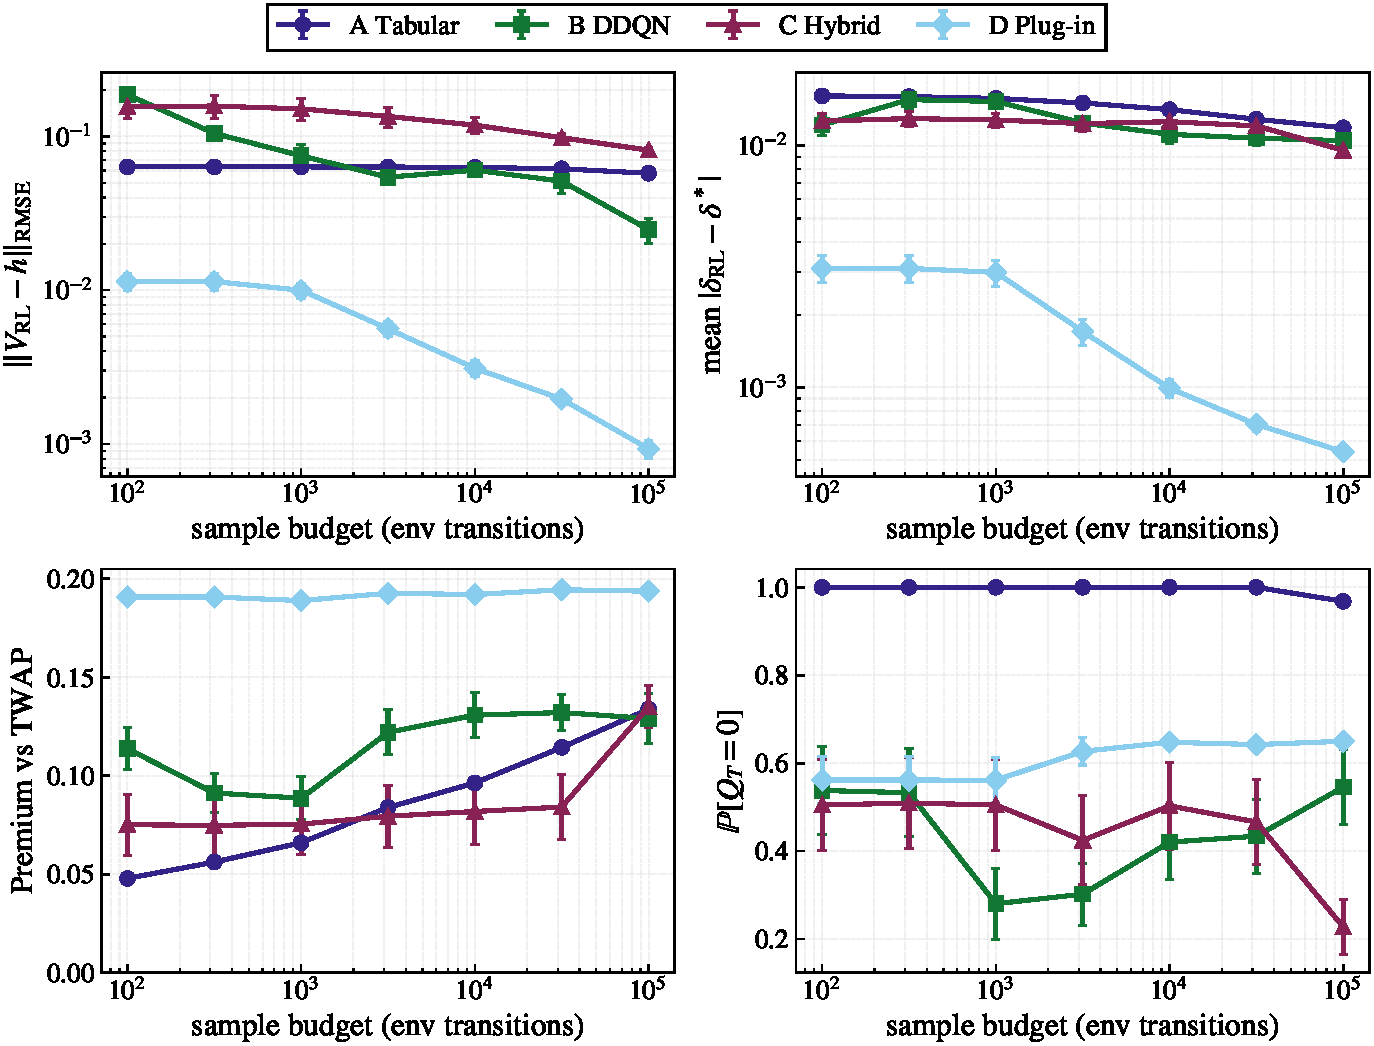
\includegraphics[width=\textwidth]{figures/fig9_sample_complexity.pdf}
\caption{Sample-complexity benchmark in the main LO+MO parameter regime, mean $\pm$ SEM over $20$ independent seeds per cell. Panel (a): RMSE of the learned value function against the FD reference $h$. Panel (b): mean absolute policy error $|\delta_{\rm RL} - \delta^*|$. Panel (c): implementation premium versus TWAP, in dollars per $10$-share liquidation episode, across $2000$ MC paths per cell. Panel (d): probability that the agent fully clears its inventory by $T$. Agent D (plug-in MLE, $\diamond$) attains essentially the FD-optimal premium at every budget; Agents A--C learn the policy from rewards alone and only catch up partially even at $n = 10^5$.}
\label{fig:fig9}
\end{figure}

The headline numbers at $n = 10^5$ appear in Table~\ref{tab:tab5}.

\begin{table}[t]
\centering
\caption{Four-agent comparison at the largest sample budget. Premium values are mean $\pm$ standard deviation across $20$ seeds; wall-clock is mean training time per seed on a single CPU core.}
\label{tab:tab5}
\begin{tabular}{@{}lcccc@{}}
\toprule
Agent & val\_err RMSE @ $10^4$ & premium @ $10^4$ & premium @ $10^5$ & wall (s) \\
\midrule
A. Tabular Q       & $0.063$ & $+0.096 \pm 0.007$ & $+0.134 \pm 0.007$ & $0.4$ \\
B. DDQN            & $0.060$ & $+0.131 \pm 0.050$ & $+0.129 \pm 0.057$ & $70.9$ \\
C. Hybrid (PPO)    & $0.118$ & $+0.082 \pm 0.075$ & $+0.135 \pm 0.048$ & $23.8$ \\
D. Plug-in MLE     & $0.003$ & $+0.192 \pm 0.006$ & $+0.194 \pm 0.007$ & $0.3$ \\
\bottomrule
\end{tabular}
\end{table}

Three observations. First, Agent D dominates the premium and value-error metrics at every budget. Once the agent's model class is correct (the CJP environment), a $\sim 100$-fill MLE plus one FD solve already attains a value-RMSE near the noise floor of the FD scheme itself. Second, Agent A (Tabular) shows the cleanest sample-complexity curve, with premium climbing to about $+0.134$ at $n = 10^5$. Third, Agent C (Hybrid PPO) becomes competitive with the model-free RL agents after the signed-residual architecture fix, but it still exhibits high run-to-run variance and remains below the plug-in premium.

We note that DDQN's premium saturates near $+0.130$ starting at $n = 10^{3.5}$ and has highly variable clearance behaviour across seeds. At $n=10^5$ its mean clearance probability is only about $0.55$ with a seed standard deviation near $0.38$, which is a stronger instability signal than the premium curve alone. This behaviour is consistent with replay-buffer overwriting and target-network drift artefacts documented in \citet[\S 5]{vanhasselt2016ddqn}; our replay buffer of $5 \times 10^4$ transitions is smaller than $n = 10^5$, so older transitions are overwritten and the effective training distribution is shifted toward the policy's late-stage behaviour. We did not pursue further hyperparameter tuning as DDQN's ceiling is well below the plug-in benchmark regardless.

The premium gap between every RL agent and the plug-in calibrator is the principal empirical result of the paper. We return to its interpretation in Section~\ref{sec:discussion}.

\subsection{Failure mode diagnostics}\label{sec:failure-modes}

Figure~\ref{fig:fig10} reports two structural failure modes diagnosed during the development of the four-agent benchmark.

\begin{figure}[t]
\centering
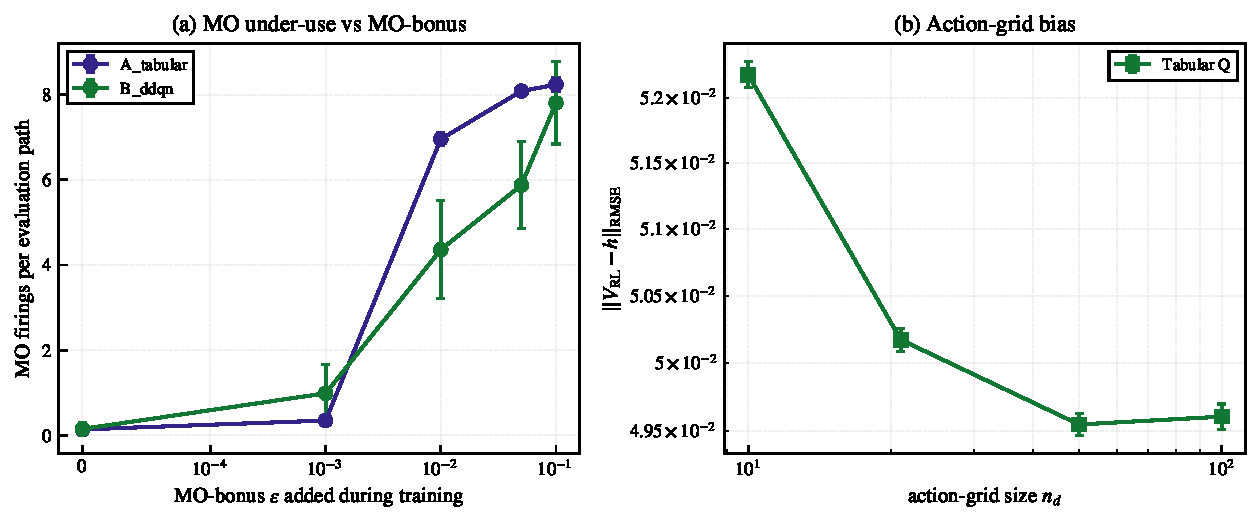
\includegraphics[width=\textwidth]{figures/fig10_failure_modes.pdf}
\caption{RL failure-mode diagnostics. Panel (a): MO firings per evaluation path as a function of an exploration $\epsilon$-bonus added to the MO action's reward during training only (evaluation uses the canonical reward of Theorem~\ref{thm:reward-shaping}). At $\epsilon = 0$, DDQN and Tabular Q both under-use MOs relative to the FD trigger, although the DDQN outcome is seed-sensitive. As the training bonus rises, both agents shift toward heavier MO use, confirming that the under-use at $\epsilon=0$ is exploration-bias driven rather than a genuine optimum. Panel (b): RMSE of the learned value function against $h$ as a function of the depth-action grid size $n_d$. Tabular Q's value error decreases only mildly as $n_d$ increases, showing that grid resolution is a secondary limiter rather than the sole source of value error.}
\label{fig:fig10}
\end{figure}

Panel (a) is the most consequential observation: agents trained on the canonical CJP reward under-sample the rare MO action under ordinary $\epsilon$-greedy exploration. Adding even a tiny per-MO bonus to the training reward (Tabular: $\epsilon \in \{10^{-3}, 10^{-2}\}$ already lifts MO use; DDQN: similar but noisier shift) demonstrates that the under-use is an exploration artefact, not a learned optimum. Hybrid Agent C uses a different exploration scheme: its MO trigger is driven by the analytic identity $h(t, q-1) - h(t, q) > \xi$ wired in through the gate logit, and the rollout policy is augmented by a forced MO-exploration probability that decays from $5\%$ to zero. To make this privilege explicit, Table~\ref{tab:forced-mo-ablation} gives Agents A and B the same decaying forced-MO hook used by Agent C.

\begin{table}[t]
\centering
\caption{Forced-MO exploration fairness ablation for Agents A and B. Runs use the Regime-I parameter set, $20$ training seeds, a $10^5$-transition-equivalent budget ($826$ training episodes), and $500$ Monte-Carlo evaluation paths per seed. Premium is mean dollars per $10$-share episode versus TWAP; ``s.e.'' is the seed-level standard error. Mean premiums differ slightly from Table~\ref{tab:tab5} because this ablation uses $500$ evaluation paths per seed whereas Table~\ref{tab:tab5} uses $2000$ paths per cell; the difference is within Monte-Carlo standard error.}
\label{tab:forced-mo-ablation}
\small
\begin{tabular}{@{}llcccc@{}}
\toprule
Agent & Exploration & Premium & s.e. & Clearance & MO/path \\
\midrule
Tabular Q & baseline $\epsilon$-greedy & $+0.140$ & $0.004$ & $0.969$ & $0.055$ \\
Tabular Q & forced MO $5\%\to0$ & $+0.135$ & $0.004$ & $1.000$ & $0.119$ \\
DDQN & baseline $\epsilon$-greedy & $+0.133$ & $0.012$ & $0.540$ & $0.028$ \\
DDQN & forced MO $5\%\to0$ & $+0.136$ & $0.010$ & $0.466$ & $0.350$ \\
\bottomrule
\end{tabular}
\end{table}

The fairness ablation does not close the calibration gap. For Tabular Q, forced MO exploration improves terminal clearance but reduces premium slightly because extra crossings give up spread. For DDQN, the hook raises MO usage and improves premium only from $+0.133$ to $+0.136$, far below the plug-in MLE's $+0.194$ in Table~\ref{tab:tab5}. Its clearance falls from $0.540$ to $0.466$ despite the higher MO count because the injected exploration distribution shifts the learned terminal-trigger timing; this is another sign of DDQN's sensitivity to the exploration distribution, not an improvement in the LO/MO trade-off. Hybrid PPO's own endpoint clearance ($0.227$ in Table~\ref{tab:tab4}) should be read in the same diagnostic spirit: wiring the analytic trigger into the gate logit does not by itself make the rare terminal MO decision reliable when the critic head that drives the trigger is still noisy. Thus Hybrid PPO's exploration privilege is a real design difference, but it does not explain the main plug-in-versus-RL premium gap. Panel (b) shows that action-grid resolution contributes only a small part of Tabular Q's value error: increasing $n_d$ from $10$ to $100$ changes RMSE by roughly $2\times10^{-3}$, so the dominant error is not merely depth discretisation.

Table~\ref{tab:tab-failure} summarises the failure modes identified in this section and the agent classes affected.

\begin{table}[t]
\centering
\caption{Summary of RL failure modes diagnosed in this paper and the agent classes they affect. \emph{Affected} = the agent class for which the failure is empirically active at default hyperparameters. \emph{Mechanism} identifies the structural reason. \emph{Mitigation} describes the patch deployed in this paper (where applicable).}
\label{tab:tab-failure}
\small
\begin{tabular}{@{}p{2.3cm}p{2.2cm}p{4.1cm}p{5.0cm}@{}}
\toprule
Failure mode & Affected & Mechanism & Mitigation \\
\midrule
MO under-use & DDQN, Tabular Q & $\epsilon$-greedy exploration starves the rare MO action & MO-action bonus during training; evaluation reward unchanged \\
Action-grid bias & Tabular Q & discrete depth grid has finite resolution & increase $n_d$, or move to continuous-action methods such as Hybrid PPO \\
MO-gate cold start & Hybrid PPO & $h_\theta$ initialised near zero gives $p_{\rm MO}^{\rm net} \approx \sigma(-\beta\xi) \approx 0$ at training start; the gate rarely fires and the agent collects little MO experience & forced $5\%$ MO-exploration probability mixed into the gate, decaying linearly to zero; A/B fairness ablation reported separately \\
\bottomrule
\end{tabular}
\end{table}

% ============================================================================
\section{Stochastic intensity extension}\label{sec:cir}
% ============================================================================

Real fill rates fluctuate. We extend the CJP framework to a CIR-type stochastic intensity \citep{coxingersollross1985,andersen2008heston}
\begin{equation}\label{eq:cir-sde}
d\lambda_t = \kappa_\lambda (\bar\lambda - \lambda_t)\, dt + \sigma_\lambda \sqrt{\lambda_t}\, dW^\lambda_t,
\end{equation}
with $W^\lambda$ independent of the midprice Brownian motion. The Feller condition $2 \kappa_\lambda \bar\lambda \ge \sigma_\lambda^2$ ensures $\lambda_t > 0$ almost surely; our default parameters $\kappa_\lambda = 2.0$, $\bar\lambda = 50/60$, $\sigma_\lambda = 0.1$ satisfy $2 \cdot 2 \cdot 50/60 \approx 3.33$, far larger than $\sigma_\lambda^2=0.01$.

\subsection{HJB on the augmented state}\label{sec:cir-hjb}
The state is now $(t, x, S, q, \lambda)$. The ansatz still simplifies the problem:

\begin{lemma}[Ansatz under CIR intensity]\label{lem:cir-ansatz}
Under \eqref{eq:midprice}--\eqref{eq:performance} with $\lambda_t$ replaced by the CIR process \eqref{eq:cir-sde}, the value function admits
$
H(t,x,S,q,\lambda) = x + q S + h(t,q,\lambda),
$
with $h(t, 0, \lambda) = 0$ for all $\lambda > 0$ and the same face-lifted terminal $h(T^-, q, \lambda) = \max\{-\alpha q^2,-q\xi\}$. The reduced function $h(t,q,\lambda)$ solves the QVI
\begin{equation}\label{eq:cir-qvi}
\begin{split}
\max\Bigl\{
&\partial_t h + \mathcal{L}_\lambda h - \phi q^2 + \frac{\ltil}{\kappa}\, e^{-\kappa[h(t,q,\lambda) - h(t,q-1,\lambda)]}\,;\\
&-\xi + h(t,q-1,\lambda) - h(t,q,\lambda) \Bigr\} = 0,
\end{split}
\end{equation}
where here $\ltil=\lambda/e$ at the current intensity and $\mathcal{L}_\lambda = \kappa_\lambda(\bar\lambda - \lambda) \partial_\lambda + \tfrac{1}{2} \sigma_\lambda^2 \lambda \partial^2_{\lambda\lambda}$ is the CIR infinitesimal generator.
\end{lemma}
\begin{proof}[Proof reference]
Apply Ito's lemma to $H$ along the controlled $(X, S, Q, \lambda)$ process; the $\lambda$-diffusion adds the $\mathcal{L}_\lambda h$ term to the HJB. Independence of $W$ and $W^\lambda$ implies the additive separability is preserved. See Appendix~\ref{app:proofs}.
\end{proof}

\subsection{Numerical scheme: upwind backward Euler}\label{sec:cir-fd}
We discretise $\lambda$ log-uniformly on $[0.5 \bar\lambda, 2 \bar\lambda]$ and augment the grid with the three validation slices $0.7\bar\lambda$, $\bar\lambda$, and $1.3\bar\lambda$; $t$ is uniform with $\Delta t = 0.05$. Each backward time step first applies an implicit backward-Euler solve for the CIR generator in $\lambda$, using a generator-form upwind stencil for the mean-reversion drift and central differences for the diffusion on the non-uniform grid. It then applies the QVI continuation/intervention update explicitly in the inventory direction. This is a first-order Lie--Trotter splitting, so the overall time accuracy is $O(\Delta t)$. Neumann boundary conditions are imposed at $\lambda_{\min}, \lambda_{\max}$; for the validated range $\sigma_\lambda \le 0.1$, the stationary CIR distribution has essentially all of its mass inside $[0.5\bar\lambda,2\bar\lambda]$, making boundary effects negligible at the reported precision. This corrected upwind direction is essential: the earlier central/incorrect-upwind variant produced non-physical large gaps at small positive $\sigma_\lambda$. With $\sigma_\lambda=0$ and $\kappa_\lambda=0$, the continuous-time problem reduces to the constant-$\lambda$ FD of Section~\ref{sec:fd}; numerically the mean slice matches that benchmark to the tolerance reported below.

\subsection{Numerical results}\label{sec:cir-results}

Figure~\ref{fig:fig11} shows three $h(t=0, q, \lambda)$ panels for $\sigma_\lambda \in \{0.0, 0.05, 0.10\}$ on a shared colour scale. The continuation value increases monotonically with $\lambda$ at every fixed $q$, reflecting that higher fill intensity makes LO posting more attractive; the three panels are visually almost indistinguishable at these moderate $\sigma_\lambda$, consistent with the $O(\sigma_\lambda^2)$ leading-order perturbation visible in Figure~\ref{fig:cirval} (next subsection).

\begin{figure}[t]
\centering
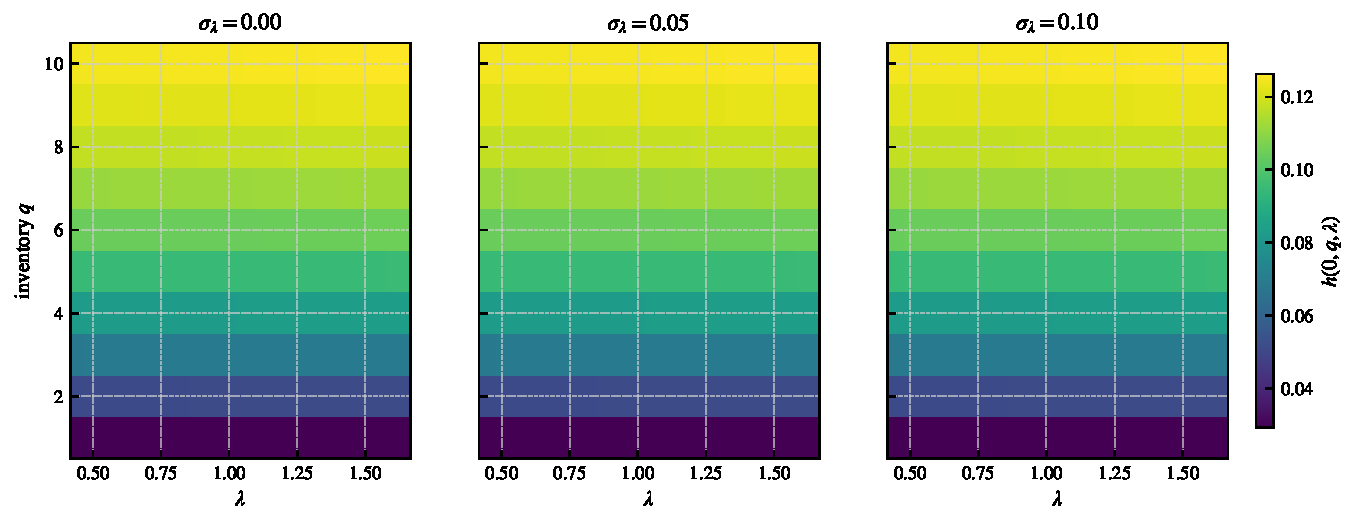
\includegraphics[width=0.95\textwidth]{figures/fig11_h_surface_cir.pdf}
\caption{Reduced value function $h(0, q, \lambda)$ under CIR-intensity dynamics for $\sigma_\lambda \in \{0,0.05,0.10\}$. The three panels share a single colour scale; the visual near-identity reflects that the leading-order stochastic-intensity correction to $h$ is small in the validated small-volatility regime. The $\sigma_\lambda=0$ panel is the deterministic-intensity sanity check.}
\label{fig:fig11}
\end{figure}

In the main LO+MO parameter regime the MO-trigger geometry collapses to an essentially one-dimensional pattern: the intervention region is active for all $q \ge 2$ at every $\lambda$ and is non-trivial only on the $q = 1$ line. A two-dimensional phase diagram therefore adds little information beyond the analytic $q \in \{1, 2\}$ result of Section~\ref{sec:q12-analytic}. The validation below restricts attention to $\sigma_\lambda \le 0.1$, where the small-volatility limit is resolved cleanly.

\subsection{Numerical validation: $\sigma_\lambda \to 0$ limit}\label{sec:cir-validation}

Figure~\ref{fig:cirval} reports a multi-slice volatility validation at $\lambda_0 \in \{0.7\bar\lambda,\bar\lambda,1.3\bar\lambda\}$. At the mean slice, $\sigma_\lambda=0$ coincides with the constant-$\lambda$ problem; away from the mean, deterministic mean reversion is already present at $\sigma_\lambda=0$, so the plotted diagnostic is $\|h_{\rm CIR}^{\sigma}(\cdot,\lambda_0,\cdot)-h_{\rm CIR}^{0}(\cdot,\lambda_0,\cdot)\|_\infty$ at the same initial intensity slice. Across all three slices, the gaps at $\sigma_\lambda \in \{0.025,0.05,0.075,0.10\}$ are approximately $8.3\times10^{-7}$, $2.8\times10^{-6}$, $5.7\times10^{-6}$, and $9.6\times10^{-6}$, respectively. Relative to $\|h_{\rm CIR}^{0}\|_\infty \approx 0.126$, these are below $8\times 10^{-5}$. The growth is approximately quadratic in $\sigma_\lambda$, consistent with the leading-order $O(\sigma_\lambda^2)$ perturbation of the deterministic-intensity ODE. This validates the small-volatility perturbation limit on and off the long-run mean; it is not a claim that the same coarse grid is validated for arbitrary high intensity volatility.

\begin{figure}[t]
\centering
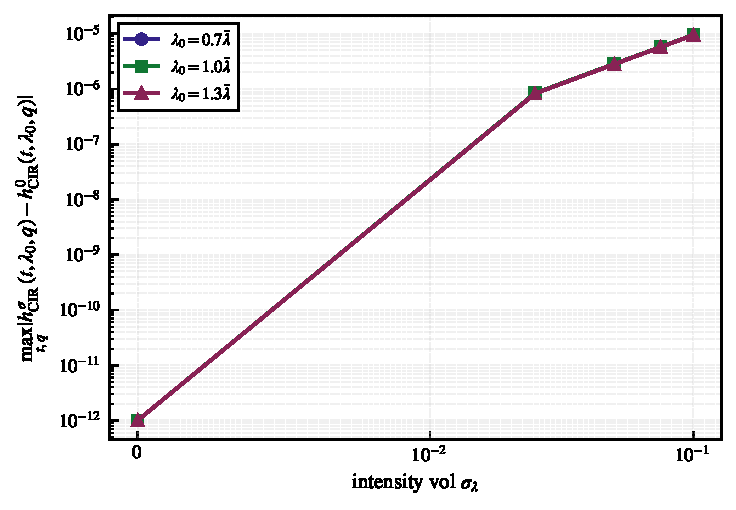
\includegraphics[width=0.62\textwidth]{figures/fig_cir_validation.pdf}
\caption{CIR scheme validation at three initial intensity slices. The plotted quantity is $\|h_{\rm CIR}^{\sigma}(\cdot,\lambda_0,\cdot)-h_{\rm CIR}^{0}(\cdot,\lambda_0,\cdot)\|_\infty$ for $\lambda_0\in\{0.7\bar\lambda,\bar\lambda,1.3\bar\lambda\}$. At the mean slice the $\sigma_\lambda=0$ reference also coincides with the constant-$\lambda$ FD solution. All positive-volatility gaps remain below $10^{-5}$ through $\sigma_\lambda=0.1$.}
\label{fig:cirval}
\end{figure}

% ============================================================================
\section{Parameter robustness and misspecification}\label{sec:robustness}
% ============================================================================

We sweep each microstructure parameter over multipliers $\{0.5, 0.75, 1.0, 1.5, 2.0\}$ of its main-regime baseline value, recompute the FD-optimal policy, and evaluate the resulting implementation premium against TWAP over $2000$ Monte-Carlo paths. Table~\ref{tab:tab6} reports the univariate sweeps.

\begin{table}[t]
\centering
\caption{Univariate parameter sensitivity. Each row varies one parameter while holding the rest at the main-regime defaults. Premium is FD-optimal versus TWAP, in dollars per $10$-share liquidation episode, over $2000$ MC paths using the robustness-script seed; small differences from the extended-baseline table reflect Monte-Carlo path-set variation.}
\label{tab:tab6}
\begin{tabular}{@{}lccccc@{}}
\toprule
Parameter $\backslash$ multiplier & $0.5$ & $0.75$ & $1.0$ & $1.5$ & $2.0$ \\
\midrule
$\lambda$ (fill rate)        & $+0.136$ & $+0.180$ & $+0.201$ & $+0.242$ & $+0.271$ \\
$\kappa$ (depth decay)       & $+0.357$ & $+0.250$ & $+0.201$ & $+0.161$ & $+0.127$ \\
$\xi$ (half-spread)          & $+0.173$ & $+0.188$ & $+0.201$ & $+0.226$ & $+0.251$ \\
$\alpha$ (terminal impact)   & $+0.200$ & $+0.205$ & $+0.201$ & $+0.203$ & $+0.198$ \\
$\phi$ (running penalty)     & $+0.215$ & $+0.203$ & $+0.201$ & $+0.207$ & $+0.205$ \\
\bottomrule
\end{tabular}
\end{table}

Economically the main directions are correct: higher $\lambda$ raises the LO premium (the agent fills faster); higher $\kappa$ erodes it (the depth-premium trade-off becomes less attractive); higher $\xi$ raises both TWAP cost and FD cost but the FD policy avoids MOs more, widening the gap. The corrected face-lift removes the spurious exact invariance in the $\alpha$ row: $\alpha$ now has a small but visible effect over factor-of-two perturbations. The small non-monotone movement in that row is within per-cell Monte-Carlo error and reflects that, at this scale, $\alpha$ is often dominated by the spread branch of the face-lift. An extreme stress test gives premiums $+0.208$, $+0.202$, $+0.185$, and $+0.185$ for $\alpha\in\{10^{-6},10^{-3},1,10^3\}$, respectively, confirming that $\alpha$ is passed through the FD solver and Monte-Carlo evaluator. The high-$\alpha$ near-invariance is expected rather than suspicious: once $\alpha q^2 \ge q\xi$, the terminal face-lift saturates at the spread branch $-q\xi$.
Figure~\ref{fig:fig-univariate} visualises the same sweeps as line plots, alongside the corresponding MO usage. With the corrected terminal face-lift, the FD policy uses MOs sparingly in the baseline regime; most of the premium response comes from the LO fill probability and the terminal face-lift trade-off rather than heavy MO intervention.

\begin{figure}[t]
\centering
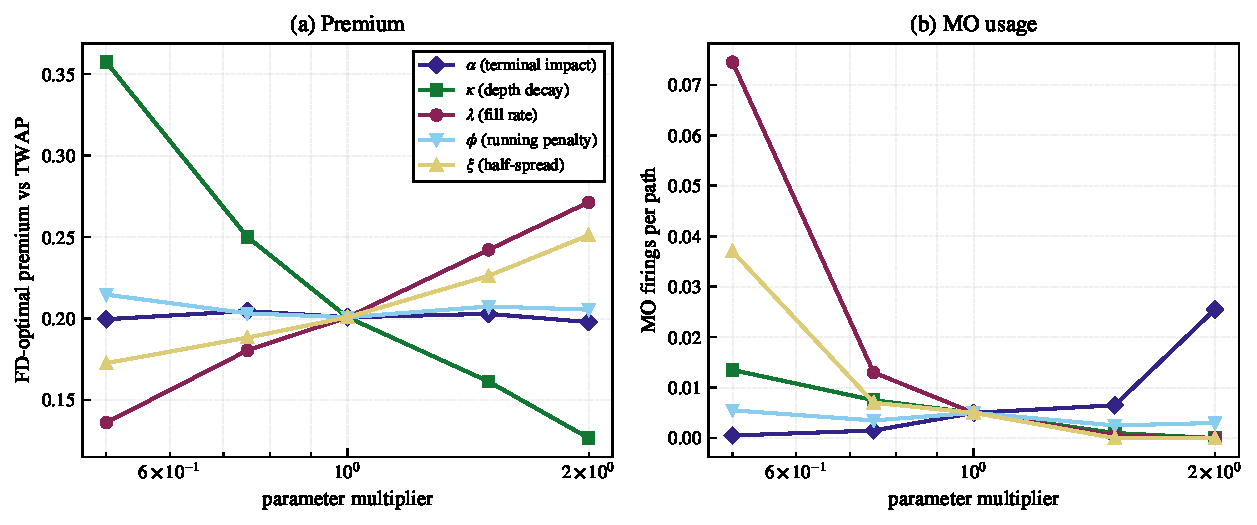
\includegraphics[width=\textwidth]{figures/fig_univariate_sensitivity.pdf}
\caption{Univariate parameter sensitivity. Panel (a): FD-optimal premium vs TWAP under each of the five microstructure parameters being scaled separately by $\{0.5, 0.75, 1, 1.5, 2\}\times$ its baseline. Panel (b): the corresponding MO-firing rate per path. The $\lambda$ and $\kappa$ sweeps produce the steepest premium responses; $\alpha$ and $\phi$ are weaker but no longer exactly invariant after the corrected terminal face-lift.}
\label{fig:fig-univariate}
\end{figure}

We additionally ran the two bivariate sweeps $(\kappa, \phi)$ and $(\xi, \alpha)$ over the same $5 \times 5$ multiplier grid; the resulting premium surfaces are dominated by single-parameter sensitivities and the numerical heatmaps are reported in Appendix~\ref{app:bivariate} for completeness. The $(\xi,\alpha)$ surface now shows small but nonzero movement along the $\alpha$ direction, as it should.

We turn instead to the most operationally relevant experiment, summarised in Figure~\ref{fig:fig16}: a $5 \times 5 \times 5 \times 5 = 625$-cell train/test misspecification grid. We train the FD-optimal policy at $(\lambda_{\rm train}, \kappa_{\rm train})$ and deploy it at $(\lambda_{\rm test}, \kappa_{\rm test})$. Panel (a) of the figure averages the realised premium across all training cells for each test cell---this is the ``what does this test cell look like if I picked a random training calibration?'' view. Panel (b) reports the more informative quantity for an execution desk: the matched-training premium (train $=$ test) minus the mean off-diagonal premium (train $\ne$ test), per cell. A positive entry means there is a genuine penalty for mis-calibration at that test cell; a near-zero entry means the FD-optimal policy is essentially calibration-insensitive there.

\begin{figure}[t]
\centering
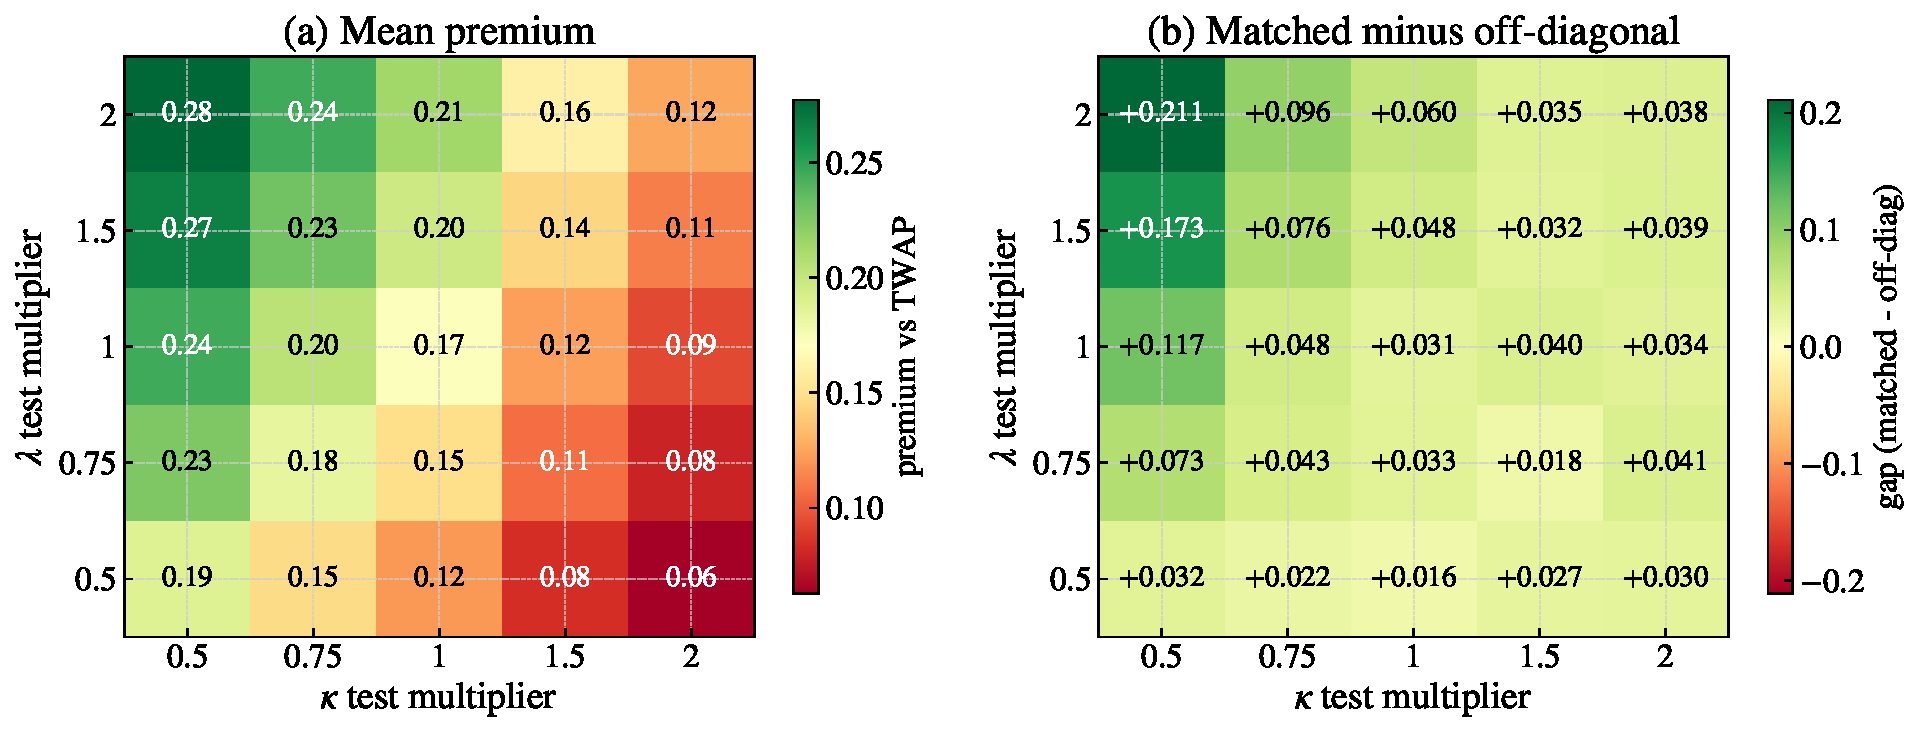
\includegraphics[width=\textwidth]{figures/fig16_robustness_misspec.pdf}
\caption{Train--test microstructure-parameter misspecification on $(\lambda, \kappa)$. Panel (a): mean premium across the $5\times 5$ training grid for each test cell; the entire grid is in the green/positive regime. Panel (b): matched-training premium minus off-diagonal-mean premium per test cell---the per-cell cost of using the wrong calibration. Cell labels are numerical premiums; the colour scale is centred at zero on the same range in both panels.}
\label{fig:fig16}
\end{figure}

Three observations from Figure~\ref{fig:fig16}. First, Panel (a) shows that every test cell sits in the positive-premium regime: the FD-optimal policy degrades gracefully under microstructure-parameter misspecification of factor $\le 2$ in either direction. Second, Panel (b) shows that the calibration sensitivity is asymmetric: cells with large $\lambda_{\rm test}$ and small $\kappa_{\rm test}$ (top-left quadrant) carry the largest matched-training advantage, while the diagonal cells of low--low and high--high parameters are nearly insensitive. Third, this robustness is the empirical underpinning of the plug-in agent's success in Section~\ref{sec:rl}: even a noisy MLE on a few hundred fills lands inside the green regime of Panel (a), so the resulting deployed policy keeps most of the FD-optimal premium.

% ============================================================================
\section{Extended baselines and statistical rigour}\label{sec:baselines}
% ============================================================================

We compare the FD-optimal and four RL agents against a panel of execution benchmarks: TWAP, Almgren--Chriss \citep{almgrenchriss2001}, VWAP (synthetic U-shape intraday volume), POV at $10\%$, a pure-passive LO at fixed depth $2/\kappa$, and a pure-aggressive policy. All baselines use the simulator-compatible interface $\pi(t, q, S) \to (\delta, \text{MO flag})$. TWAP here is the simulator-faithful constant unit-MO baseline; alternative batched TWAP implementations would shift absolute premiums but not the policy-diagnostic comparisons below. Each premium claim in this paper is accompanied by a paired-bootstrap $95\%$ confidence interval with $10^4$ replicates; cross-seed aggregates use the percentile bootstrap on the $20$ seed-level means.

Table~\ref{tab:tab4} reports the full panel. Two observations. First, the deterministic schedule baselines (Almgren--Chriss, VWAP, POV) cluster close to TWAP, confirming that under the CJP environment with our calibrated parameters the main premium source is access to passive LO fills rather than deterministic schedule reshuffling. Pure aggressive is not statistically distinguishable from TWAP because its confidence interval crosses zero. Second, pure-passive LO at fixed depth $2/\kappa$ already earns a large premium because it avoids paying the half-spread on most shares; its weakness is not price but completion, with only $14\%$ of paths fully cleared before the terminal face-lift. The FD-optimal policy improves on pure passive by adapting depth and terminal liquidation, but it does not mechanically force $Q_T=0$ on every path because the corrected face-lift sometimes makes a small terminal block liquidation cheaper than late market orders. Pure aggressive records fewer than ten MOs per path because, in the simulator-compatible interface, it still posts a zero-depth LO in steps where an MO is sent; occasional external fills after the agent MO reduce the remaining number of crossing trades.

\begin{table}[t]
\centering
\caption{Extended baseline panel in the main LO+MO parameter regime, $n_{\rm paths} = 2000$ Monte-Carlo evaluation paths, seed $42$. Baseline rows use deterministic policies, so single-seed evaluation plus paired bootstrap captures Monte-Carlo uncertainty; agent rows use the cross-seed protocol from Table~\ref{tab:tab5}. Premium values are mean of (terminal value of strategy) $-$ (terminal value of TWAP), in dollars per $10$-share episode, with paired-bootstrap $95\%$ CI in brackets. $\mathbb{P}[Q_T = 0]$ is the empirical pre-terminal clearance probability; \#MO is the mean number of agent market orders per path where stored by the baseline evaluator.}
\label{tab:tab4}
\begin{tabular}{@{}lccc@{}}
\toprule
Strategy & Premium vs TWAP & $\mathbb{P}[Q_T = 0]$ & \#MO/path \\
\midrule
TWAP (reference)              & $0$ (def.)               & $1.000$ & $10.00$ \\
Almgren--Chriss ($\eta=0.05$) & $-0.0042$ $[-0.012,\!+0.003]$ & $1.000$ & $10.00$ \\
VWAP (U-shape)                & $-0.0008$ $[-0.003,\!+0.002]$ & $1.000$ & $10.00$ \\
POV at $10\%$                 & $+0.0054$ $[-0.004,\!+0.015]$ & $1.000$ & $5.00$ \\
Pure passive ($\delta = 2/\kappa$) & $+0.1605$ $[+0.129,\!+0.192]$ & $0.141$ & $0.00$ \\
Pure aggressive (immediate MO)& $-0.0071$ $[-0.027,\!+0.013]$ & $1.000$ & $9.64$ \\
\midrule
FD Optimal                    & $+0.1859$ $[+0.159,\!+0.214]$ & $0.642$ & $0.00$ \\
D. Plug-in MLE ($n = 10^5$)   & $+0.1937 \pm 0.007$         & $0.650$ & --- \\
\midrule
A. Tabular Q ($n = 10^5$)     & $+0.1338 \pm 0.007$         & $0.968$ & --- \\
B. DDQN ($n = 10^5$)          & $+0.1290 \pm 0.057$         & $0.546$ & --- \\
C. Hybrid PPO ($n = 10^5$)    & $+0.1350 \pm 0.048$         & $0.227$ & --- \\
\bottomrule
\end{tabular}
\end{table}

Because the experiment CSVs store seed-level endpoint summaries rather than path-level terminal-wealth series, we report paired seed-level endpoint comparisons in Appendix~\ref{app:pairwise-stats} instead of a path-level Diebold--Mariano matrix. The qualitative message is unchanged: the adjacent RL agents are not statistically separable by premium, while the Regime-I gap from the RL group to the plug-in MLE is stable.

\subsection{Institutional-scale stress test}\label{sec:regime-ii}

To test whether the pure-passive result above is only a small-scale artefact, we repeat the comparison at $Q_0=100$ and $T=600$s with the scaled parameters stated in the model section. The next figure reports the Regime-II sample-complexity curves; the following table reports the endpoint comparison.

For interpretation, separate the terminal-wealth premium reported in the baseline tables from the QVI-consistent shaped objective. Suppressing the martingale midprice terms, the latter decomposes as
\[
\E\!\left[\sum_{\text{LO fills}}\delta_i
- \xi\, \#\text{MO}
- \phi\int_0^T Q_s^2\,ds
- \min\{\alpha Q_T^2,\xi Q_T\}\right].
\]
Thus a policy can display a high raw terminal-wealth premium by waiting for passive fills while still being suboptimal for the QVI because it accumulates running inventory cost or leaves a costly terminal block.

\begin{figure}[t]
\centering
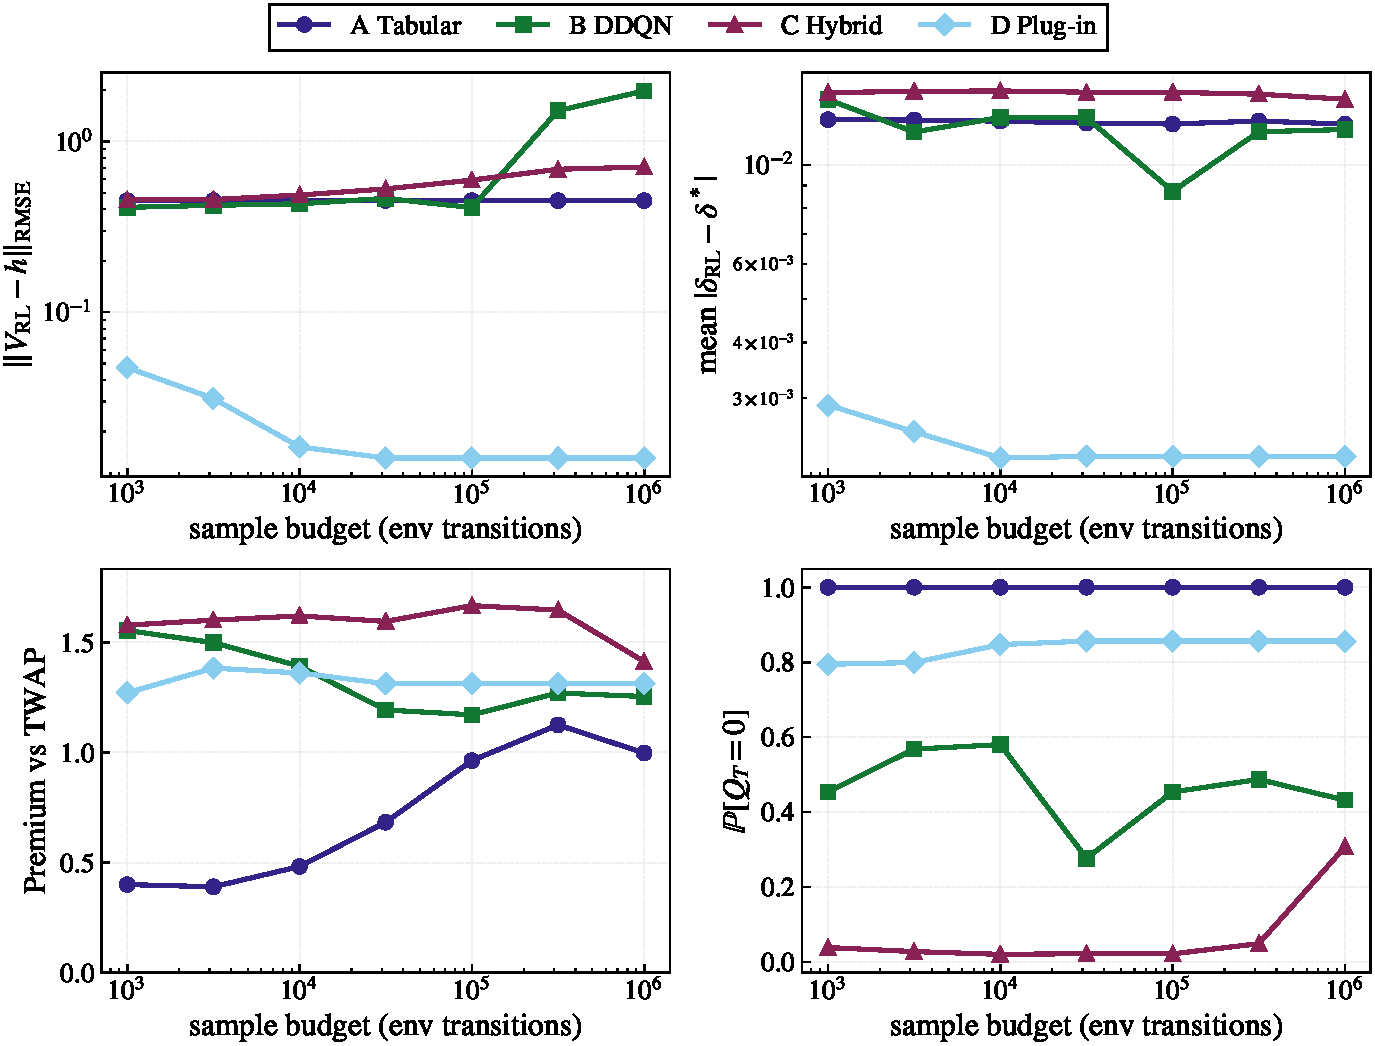
\includegraphics[width=\textwidth]{figures/fig_regime_ii_sample_complexity.pdf}
\caption{Regime-II sample-complexity stress test ($Q_0=100$, $T=600$s). Each point averages $20$ training seeds and $500$ Monte-Carlo evaluation paths per seed. Unlike the Regime-I panel, cash premium alone is not monotone in value accuracy: DDQN and Hybrid PPO sometimes post high cash premium by remaining passive, but their value RMSE and clearance metrics reveal that they are not solving the FD objective as accurately as Plug-in MLE.}
\label{fig:regime-ii-sc}
\end{figure}

\begin{table}[t]
\centering
\caption{Regime-II endpoint comparison. Baseline rows use deterministic policies and $2000$ paired Monte-Carlo paths; agent rows use the $n=10^6$ sample-complexity endpoint, $20$ seeds, and $500$ evaluation paths per seed. The uncertainty shown for agents is the seed-level standard deviation of premium. The plug-in baseline row is evaluated under the baseline-panel protocol, while the plug-in endpoint row is the sample-complexity endpoint under the 20-seed protocol, so the two rows should not be read as a monotone fill-budget comparison. Premium is dollars per $100$-share episode relative to TWAP.}
\label{tab:regime-ii}
\small
\begin{tabular}{@{}lccc@{}}
\toprule
Strategy & Premium vs TWAP & $\mathbb{P}[Q_T=0]$ & Diagnostic \\
\midrule
Pure passive              & $+0.785$ $[-0.228,\!+1.751]$ & $0.000$ & $67.38$ LO/path \\
FD Optimal                & $+0.975$ $[+0.273,\!+1.631]$ & $0.857$ & $30.64$ MO/path \\
Plug-in baseline ($1000$ fills)& $+0.958$ $[+0.239,\!+1.638]$ & $0.862$ & FD-matching \\
\midrule
A. Tabular Q ($n=10^6$)   & $+0.998 \pm 0.565$ & $1.000$ & RMSE $0.450$ \\
B. DDQN ($n=10^6$)        & $+1.254 \pm 0.640$ & $0.432$ & RMSE $1.974$ \\
C. Hybrid PPO ($n=10^6$)  & $+1.413 \pm 0.668$ & $0.307$ & RMSE $0.707$ \\
D. Plug-in endpoint ($n=10^6$) & $+1.312 \pm 0.396$ & $0.856$ & RMSE $0.014$ \\
\bottomrule
\end{tabular}
\end{table}

Figure~\ref{fig:regime-ii-pareto} visualises the same endpoint as a multi-objective comparison rather than a single cash-premium ranking.

\begin{figure}[t]
\centering
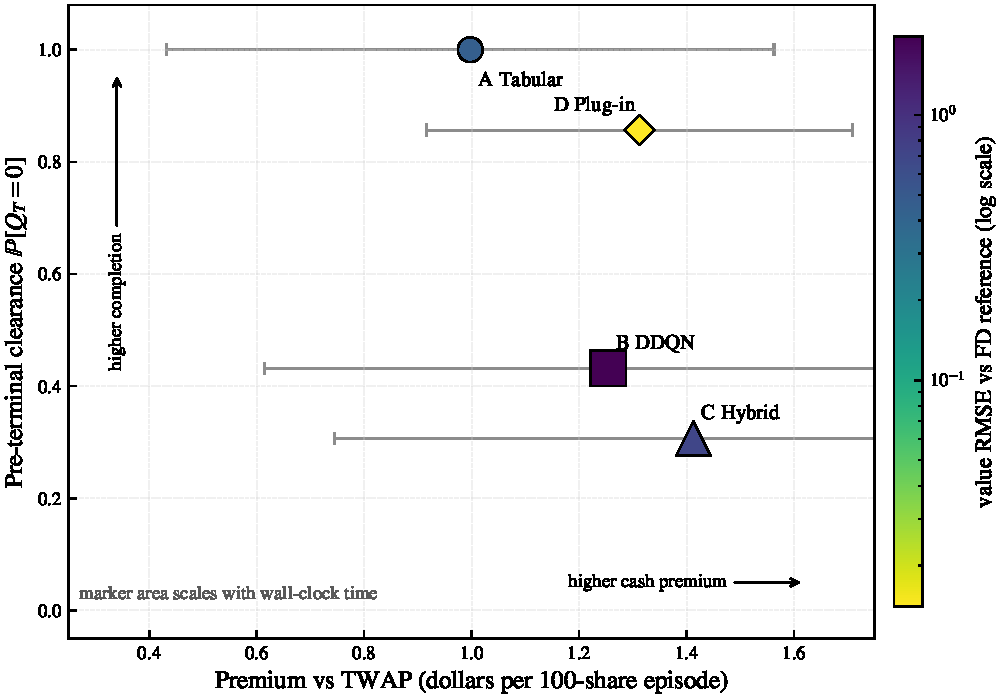
\includegraphics[width=0.85\textwidth]{figures/fig_regime_ii_pareto.pdf}
\caption{Regime-II endpoint multi-metric view at $n=10^6$. The horizontal axis is raw terminal-cash premium, the vertical axis is pre-terminal clearance, colour gives value RMSE against the FD reference on a log scale, and marker area scales with mean wall-clock time (A: $4.7$s, B: $729$s, C: $381$s, D: $0.56$s). Hybrid PPO has the largest cash-premium point estimate, but it sits in a low-clearance, high-RMSE, high-compute region; Plug-in MLE is not the largest-premium point but is simultaneously close to the upper-right completion region, has the lowest value error, and is computationally negligible.}
\label{fig:regime-ii-pareto}
\end{figure}

The stress test closes a specific loophole in the Regime-I narrative but also rules out an overly simple ``calibration always has the largest cash premium'' claim. Pure passive still earns positive cash premium because avoiding the half-spread is valuable, but it never clears pre-terminal inventory in our $2000$-path run and is overtaken by FD Optimal and Plug-in MLE. Its QVI weakness becomes much larger at scale: the rough running-penalty magnitude $\phi Q_0^2T$ rises from $10^{-5}\cdot10^2\cdot60\approx0.06$ in Regime I to $10^{-6}\cdot100^2\cdot600\approx6$ in Regime II. The FD-optimal point estimate is below several agent point estimates only because the evaluation protocols and Monte-Carlo path sets differ; its paired bootstrap interval $[+0.273,+1.631]$ covers the learned-agent means, consistent with FD optimality at the matched parameters. Among learned agents, Hybrid PPO posts the largest cash-premium point estimate ($+1.413$), and DDQN sits just below the plug-in endpoint ($+1.254$ versus $+1.312$), but the seed-level ordering is weak: paired bootstrap differences versus the plug-in endpoint are $-0.058$ for DDQN (95\% CI $[-0.349,+0.232]$) and $+0.100$ for Hybrid PPO (95\% CI $[-0.265,+0.447]$). These are not statistically distinguishable from zero. The value-RMSE diagnostic is by construction more favourable to Plug-in MLE than to model-free agents, because Plug-in plans by FD at fitted parameters and therefore inherits the FD scheme's accuracy as $|\hat\kappa-\kappa|+|\hat\lambda-\lambda|\to0$. Its diagnostic content is therefore not that Plug-in matches FD by tautology, but that the model-free agents do not approach the value function at the tested budget; the latter remains a meaningful operational gap. The mechanism is still informative: higher raw premium comes from more patient passive exposure and LO income, while the high RMSE and low clearance show accumulated running-cost and face-lift risk. We therefore read Regime II as a scale-dependent result: model-free RL can produce aggressive cash-premium heuristics at larger scale, but the calibrated FD policy remains the only method that is simultaneously accurate against the QVI, computationally cheap, and completion-stable.

% ============================================================================
\section{Discussion}\label{sec:discussion}
% ============================================================================

\subsection{Economic implications}\label{sec:econ-implications}
The principal economic message is scale-dependent and model-class dependent. Within the assumptions of the present CJP model class and at the small Chapter~8 inventory scale $Q_0=10$, devoting compute to fitting $(\hat\kappa, \hat\lambda)$ and solving the FD QVI on the calibrated parameters dominates devoting compute to neural-network policy training. Our Plug-in MLE agent's premium at $n = 10^5$ remains materially above DDQN's at the same budget, and the gap does not vanish with more training.

The Regime-II stress test changes the operational interpretation. At $Q_0=100$, learned agents can have larger terminal-cash point estimates than the plug-in benchmark, but the paired seed-level uncertainty is wide and their value-function errors and completion rates show that this is not the same as solving the CJP liquidation objective accurately. For a real execution desk this argues for reporting at least three metrics---cash premium, QVI/value error, and pre-terminal clearance---rather than judging execution RL only by terminal-value premium. It also supports periodic re-calibration over end-to-end RL when the CJP microstructure is a reasonable local approximation: the calibrated policy is not always the largest raw-premium row, but it is the stable FD-matching row with negligible training cost.

The CIR-intensity extension (Section~\ref{sec:cir}) reveals a richer picture. The QVI of Lemma~\ref{lem:cir-ansatz} makes the dependence of the continuation value on the realised $\lambda_t$ explicit: at low $\lambda$ the expected LO-fill rate is lower, so the trade-off between waiting, firing MOs, and accepting the terminal face-lift shifts. A desk that ignores intensity stochasticity and uses the constant-$\lambda$ FD policy posts depths calibrated to $\bar\lambda$; on realised paths with $\lambda_t<\bar\lambda$, this under-fills, leaves larger terminal residuals, and incurs more face-lift cost.

\subsection{Methodological implications}\label{sec:method-implications}
The reward shaping of Theorem~\ref{thm:reward-shaping} is, to our knowledge, the first cleanly published characterisation of a CJP-compatible reward whose expectation coincides with the analytic value function. It generalises to any control problem with an additive value decomposition $H = (\text{linear in state}) + h(t, q)$, making the pointwise diagnostic $\|V_{\rm RL} - h\|_\infty$ available as a correctness check for any model-free agent. We expect this construction to be useful for the optimal market-making literature \citep{avellanedastoikov2008, gueant2012inventory, spooner2018mm} and the model-uncertainty-robust execution literature \citep{cartea2017uncertainty}.

The structure-aware hybrid (Agent C) is, in retrospect, the most informative negative result of our benchmark. Its architecture hard-wires two pieces of CJP structure---the $\kappa^{-1}$ depth asymptote and the analytic MO trigger condition $h(t,q-1) - h(t,q) > \xi$---and its parameter count ($\approx 350$) is one-fifteenth of DDQN's. We explicitly remove the softplus floor that would force $\delta\ge \kappa^{-1}$: the residual head is signed and can quote below the asymptote. After this architectural correction, Hybrid roughly matches Tabular Q within seed-level noise in Regime I, suggesting that the architectural prior compensates for some but not all of PPO's overhead. It remains high variance on the rare-event MO gate: at $n=10^5$ the seed-level premium standard deviation is about $0.048$, roughly seven times the plug-in calibrator's $0.007$, and terminal clearance is only $0.227$. It therefore does not match the plug-in calibrator within the tested budgets. Thus the negative result should be read as a statement about the training route in this CJP-faithful benchmark, not as proof that all structure-aware policies must fail.

The implication for execution RL practitioners is that, when the analytic structure of the problem is rich enough to identify a small parametric family (as is the case for CJP), the productive use of compute is often parameter calibration plus analytical solving, not end-to-end policy learning. This conclusion should be read as a model-based RL statement: a correct low-dimensional model plus planning is hard for model-free learners to beat on sample efficiency, whereas structure-aware deep-learning designs may be more valuable when the model class itself is partially misspecified (e.g., LOB-feature-conditional execution), a setting we leave to future work.

\subsection{Limitations}\label{sec:limitations}
We acknowledge the following limitations.
\begin{enumerate}
\item The midprice is an arithmetic Brownian motion, not a jump-diffusion or a rough volatility process; the LO/MO dynamics inherit the standard CJP simplifications.
\item We consider a single asset; cross-asset hedging and basket-execution interactions are not addressed.
\item External order flow is exogenous: the agent has no self-impact on $\lambda$. \citet{alfonsi2016hawkes} treat the Hawkes self-exciting case; we leave RL on that environment for future work.
\item The half-spread $\xi$ is constant; queue-position dynamics and adverse selection are not modelled.
\item We do not include every modern continuous-action RL baseline. Soft Actor-Critic \citep{haarnoja2018sac}, distributional RL, and nonparametric model-based RL are natural extensions; our present comparison focuses on DDQN because of its direct connection to the execution benchmark of \citet{ninglinjaimungal2021}, and on PPO because it implements the structure-aware continuous-depth hybrid.
\item The main sample-complexity benchmark uses the CJP Chapter~8 pedagogical scale $Q_0=10$. Section~\ref{sec:regime-ii} adds a $Q_0=100$ stress test, but true institutional liquidations can be orders of magnitude larger; extending the benchmark to $Q_0=10^3$--$10^6$ requires either coarser state aggregation or asymptotic scaling arguments.
\item Beyond the CIR intensity studied here, more realistic intensity dynamics (Hawkes, regime-switching, jump-diffusion) are out of scope.
\item We validate everything in simulation; a real LOB-data validation in the style of \citet{karpe2020abides} is reserved for follow-on work.
\end{enumerate}

% ============================================================================
\section{Conclusion}\label{sec:conclusion}
% ============================================================================

We have constructed a sample-complexity benchmark for CJP optimal liquidation that compares model-free RL, structure-aware RL, and plug-in parametric model-based planning on a common simulator with a common reward-shaped MDP whose return equals the reduced value function. At the CJP Chapter~8 scale, the central empirical finding is that a two-parameter MLE plus one FD solve dominates every model-free agent we evaluate, including Double DQN with $\sim 5\,000$ parameters trained on $10^5$ environment transitions, and that this gap does not close with sample budget. At the $Q_0=100$ stress-test scale, the ranking by cash premium becomes less monotone and statistically noisy, but Plug-in MLE remains the FD-matching, completion-stable, and computationally cheap method. A structure-aware hybrid policy that hard-wires the CJP asymptote into its architecture can have a larger raw-premium point estimate at the larger scale, but it does not match the plug-in calibrator's value accuracy or completion stability.

A CIR-type stochastic intensity extension confirms the $\sigma_\lambda\to0$ limit on $\sigma_\lambda \in [0,0.1]$ after correcting the upwind discretisation of the intensity generator. A $625$-cell microstructure-parameter misspecification study shows the FD policy degrades gracefully under factor-of-two parameter errors, which is the empirical reason the noisy $100$-fill MLE works.

The picture that emerges is that, when the model class is broadly correct, machine learning's role in execution may be parameter calibration plus analytical solving rather than end-to-end policy training. The Regime-II stress test qualifies this statement: learned policies can tilt the cash-premium metric upward in noisy seed means, but doing so exposes the need to report value accuracy and clearance alongside premium. The most natural extensions of this work involve environments where the CJP model class fails: Hawkes self-exciting intensities \citep{alfonsi2016hawkes}, LOB-feature-conditional execution \citep{ninglinjaimungal2021}, real LOB data with adverse selection \citep{karpe2020abides}, nonparametric model-based RL, and multi-asset basket liquidation. We conjecture that the calibration-versus-RL trade-off pivots in exactly these regimes, and benchmarking that pivot is the natural follow-on.

% ============================================================================
\section*{Acknowledgments}
The author thanks Professors Weiming Ni, Xingbin Pan, Yang Liu, and Gongqiu Zhang of the School of Science and Engineering, The Chinese University of Hong Kong, Shenzhen, for their teaching and guidance. Professor Ni's rigorous and careful teaching strengthened the author's mathematical training; Professor Pan's courses were formative in inspiring the author's interest in mathematics; Professors Liu and Zhang provided valuable instruction in related mathematical and financial mathematics coursework.

\section*{Disclosure statement}
The author has prior internship experience in quantitative trading; the relevant firm provided no data, compute, supervision, or input on this work. The firm name is available to the editor for conflict-of-interest review. The author reports no other conflict of interest.

\section*{Funding}
No external funding supported this work.

\section*{Data availability statement}
All Monte-Carlo seeds, finite-difference solution grids, and intermediate CSVs are available in the project repository at \url{https://github.com/VernonOY/amf-cjp-liquidation-benchmark}, which will be archived with a persistent DOI upon acceptance. The single command \texttt{bash run\_all.sh all} reproduces every figure and table in this paper end-to-end ($\approx 8$ hours on a 12-core CPU). A lighter command, \texttt{bash run\_all.sh phase1}, runs only the golden-snapshot regression tests ($\approx 5$ minutes), while selected experiment targets accept a \texttt{--smoke} option for small sanity checks. The experiment scripts \texttt{exp1\_sample\_complexity.py}, \texttt{exp1\_regime\_cached.py}, \texttt{exp2\_stochastic\_lambda.py}, \texttt{exp3\_robustness.py}, \texttt{exp4\_failure\_modes.py}, and \texttt{exp5\_regime\_baselines.py} are individually invocable for partial reproduction.

% ============================================================================
\appendix

\section{Proofs}\label{app:proofs}

\subsection{Proof of Proposition~\ref{prop:ansatz}}
Write the wealth process $X^{\delta,M}_t$ in terms of LO fills and MO impulses as in \eqref{eq:cashsde}. For any admissible $(\delta, M)$, the inventory $Q_t$ is bounded by $Q_0$ and the midprice has finite second moment, so $\E[Q_T S_T] = q S_t$ by the martingale property of $S$. The terminal payoff in \eqref{eq:performance} decomposes additively into the cash component $X_T$ (a martingale increment from $X_t = x$) plus the inventory liquidation value $Q_T (S_T - \alpha Q_T)$ plus the running cost. Taking essential supremum and using that the cash and midprice contributions are independent of the agent's control choice $(\delta, M)$ \emph{conditional} on the realised path, yields $H(t,x,S,q) = x + qS + h(t,q)$ with $h$ depending only on $(t, q)$. The pre-terminal face-lift follows by comparing terminal block liquidation to firing unit MOs.

\subsection{Proof of Theorem~\ref{thm:reward-shaping}}
Fix an admissible policy $\pi$ and write its reduced value as $h^\pi$. Under the ansatz \eqref{eq:ansatz},
\[
h^\pi(t,q)
= \E_\pi\!\left[
X_T-X_t + Q_T S_T - qS_t
-\phi\int_t^T Q_s^2\,ds
-\min\{\alpha Q_T^2,\xi Q_T\}
\,\middle|\, Q_t=q\right],
\]
where the terminal term uses the same face-lift convention as the QVI. The cash and inventory dynamics imply, pathwise over the LO/MO jump times,
\[
dX_s + S_{s^-}\,dQ_s = \delta_{s^-}\,dN_s^\delta - \xi\,dM_s.
\]
Moreover, since $S$ is a continuous semimartingale and $Q$ is purely discontinuous, $[Q,S]=0$ and Ito's product rule gives
$d(Q_sS_s)=Q_{s^-}\,dS_s+S_{s^-}\,dQ_s$ exactly. The stochastic integral $\int_t^T Q_{s^-}\,dS_s$ has zero expectation because $S$ is a martingale and $Q$ is bounded: indeed $|Q_s|\le Q_0$ and $d\langle S\rangle_s=\sigma^2ds$ imply $\E[\int_t^T Q_{s^-}^2\,d\langle S\rangle_s]\le Q_0^2\sigma^2T<\infty$. Therefore
\[
\E_\pi[X_T-X_t+Q_T S_T-qS_t]
=\E_\pi\!\left[\sum_{\text{LO fills}}\delta_s-\xi\,\#\text{MO}\right].
\]
Substituting this identity into the reduced payoff gives
\[
h^\pi(t,q)
=\E_\pi\!\left[
\sum_{\text{LO fills}}\delta_s
-\xi\,\#\text{MO}
-\phi\int_t^T Q_s^2\,ds
-\min\{\alpha Q_T^2,\xi Q_T\}
\,\middle|\, Q_t=q\right],
\]
which is exactly the continuous-time cumulative reward associated with \eqref{eq:reward}. The discrete simulator replaces the integral by the left-continuous Riemann sum $\sum Q_{t^-}^2\Delta t$, giving the stated $O(\Delta t)$ approximation. Taking the supremum over $\pi$ yields $J^{\pi^*}=h$.

\subsection{Proof of Lemma~\ref{lem:cir-ansatz}}
By independence of $W^\lambda$ and $W$, Ito on $H$ along $(X, S, Q, \lambda)$ adds the $\mathcal{L}_\lambda h$ term to the HJB without coupling $\lambda$ to $S$. Linearity of $H$ in $(x, S)$ is preserved because the additional drift acts only on the $h$ component.

\section{RL implementation details}\label{app:rl-details}

\subsection{Hybrid policy architecture (Agent C)}\label{app:hybrid-arch}
The network has two hidden layers of $16$ units each with $\tanh$ activations, followed by three heads: $g_\theta$ (depth residual, one output), $h_\theta$ (value, one output), and $\log\beta$ (scalar trainable parameter). The residual is signed and bounded as
$
g_\theta = 0.025(1+\tanh(\tilde g_\theta))-0.01 \in [-0.01,0.04],
$
so the depth mean $\delta = \kappa^{-1} + g_\theta$ can move below $\kappa^{-1}$ and reach the zero-depth grid point after snapping. The numerical bounds are scaled to the $\kappa=100$ regimes studied here; for materially different $\kappa$ one should rescale the residual window with $\kappa^{-1}$ rather than reuse the absolute interval. The MO trigger probability is $\sigma(\beta \cdot [(h_\theta(t, q-1) - h_\theta(t, q)) - \xi])$. At rollout, exploration noise $\mathcal{N}(0, \sigma_{\rm explore})$ is added to the continuous depth and snapped to the env's discrete depth grid using a categorical Gaussian-density softmax; this preserves a differentiable log-prob. Training also uses a linearly decaying forced MO-exploration probability from $5\%$ to zero.

\subsection{PPO update}\label{app:ppo}
For each batch of episodes we recompute log-probabilities of all stored $(s, a)$ pairs under the current network, form the clipped surrogate objective
$
\mathcal{L}_{\rm CLIP}(\theta) = -\E\left[ \min\bigl( r_t(\theta) A_t,\ \text{clip}(r_t(\theta), 1 - \epsilon, 1 + \epsilon) A_t \bigr) \right],
$
add a value loss $c_v \|h_\theta - G_t\|^2$ with $c_v = 5$, and do $4$ Adam updates per batch with learning rate $3 \times 10^{-4}$. The clip parameter is $\epsilon = 0.2$. Advantage $A_t = G_t - h_\theta(s_t)$ is normalised to unit variance before clipping.

\subsection{Plug-in MLE (Agent D)}\label{app:plugin}
The exact-Bernoulli log-likelihood is maximised in log-domain $(\log \lambda, \log \kappa)$ via L-BFGS-B with a weak Gaussian prior $\mathcal{N}(\log \lambda_0, \sigma_p)$ and similarly for $\kappa$. The tight prior $\sigma_p = \log 2$ is used when fewer than $200$ fills have been observed; the loose prior $\sigma_p = \log 10$ otherwise. In the sample-complexity plots, the horizontal axis is an environment-transition budget for all agents; for Agent D this budget is converted into a target fill count using the exploration policy's expected fill rate, with a small floor to avoid degenerate likelihoods and a $1000$-fill cap in Regime II. Once $(\hat\kappa, \hat\lambda)$ is in hand, the standard FD solver of Section~\ref{sec:fd} is invoked once at the estimated parameters, and the resulting policy is deployed without further updates.

\section{Bivariate sensitivity sweeps}\label{app:bivariate}

The bivariate sweeps referenced in Section~\ref{sec:robustness} are reported here as numeric tables. Each cell is the FD-optimal premium versus TWAP at the perturbed parameters, $2000$ Monte-Carlo paths per cell, seed $0$. Premium values are reported to three decimal places.

\begin{table}[h]
\centering
\caption{Bivariate $(\kappa, \phi)$ sweep. Rows: $\kappa$ multiplier; columns: $\phi$ multiplier. Premium is FD-optimal vs TWAP.}
\label{tab:appB-kphi}
\begin{tabular}{@{}lccccc@{}}
\toprule
$\kappa \backslash \phi$ & $0.50$ & $0.75$ & $1.00$ & $1.50$ & $2.00$ \\
\midrule
$0.50$ & $+0.351$ & $+0.358$ & $+0.357$ & $+0.347$ & $+0.343$ \\
$0.75$ & $+0.255$ & $+0.257$ & $+0.250$ & $+0.246$ & $+0.251$ \\
$1.00$ & $+0.215$ & $+0.203$ & $+0.201$ & $+0.207$ & $+0.205$ \\
$1.50$ & $+0.153$ & $+0.154$ & $+0.161$ & $+0.146$ & $+0.150$ \\
$2.00$ & $+0.125$ & $+0.139$ & $+0.127$ & $+0.122$ & $+0.117$ \\
\bottomrule
\end{tabular}
\end{table}

\begin{table}[h]
\centering
\caption{Bivariate $(\xi, \alpha)$ sweep. Rows: $\xi$ multiplier; columns: $\alpha$ multiplier. The corrected face-lift produces small but nonzero variation along the $\alpha$ axis.}
\label{tab:appB-xialpha}
\begin{tabular}{@{}lccccc@{}}
\toprule
$\xi \backslash \alpha$ & $0.50$ & $0.75$ & $1.00$ & $1.50$ & $2.00$ \\
\midrule
$0.50$ & $+0.175$ & $+0.176$ & $+0.173$ & $+0.175$ & $+0.175$ \\
$0.75$ & $+0.187$ & $+0.192$ & $+0.188$ & $+0.188$ & $+0.185$ \\
$1.00$ & $+0.200$ & $+0.205$ & $+0.201$ & $+0.203$ & $+0.198$ \\
$1.50$ & $+0.225$ & $+0.230$ & $+0.226$ & $+0.224$ & $+0.220$ \\
$2.00$ & $+0.250$ & $+0.255$ & $+0.251$ & $+0.249$ & $+0.246$ \\
\bottomrule
\end{tabular}
\end{table}

The $(\kappa, \phi)$ table shows that premium is dominated by the $\kappa$ row index while the within-row variation across $\phi$ is much smaller. The $(\xi,\alpha)$ table is similarly dominated by $\xi$, but the $\alpha$ direction is no longer exactly flat.

\section{Seed-level pairwise endpoint statistics}\label{app:pairwise-stats}

The main experiment stores one aggregate row per training seed. The tables below therefore compare endpoint seed means rather than path-level terminal-wealth losses. For each pair, we align common seed indices, report the mean premium difference (first agent minus second agent), a percentile-bootstrap 95\% confidence interval over seeds, the paired $t$-test $p$-value, and a Holm-corrected $p$-value across the six pairwise comparisons in that regime.

\begin{table}[h]
\centering
\caption{Regime-I pairwise seed-level premium differences at $n=10^5$. Positive values favour the first agent in the comparison.}
\label{tab:pairwise-regime-i}
\small
\begin{tabular}{@{}lrrrr@{}}
\toprule
Comparison & Mean diff. & 95\% CI & $p$ & Holm $p$ \\
\midrule
A Tabular $-$ B DDQN & +0.005 & $[-0.019,+0.031]$ & 0.720 & 1.000 \\
A Tabular $-$ C Hybrid & -0.001 & $[-0.021,+0.021]$ & 0.911 & 1.000 \\
A Tabular $-$ D Plug-in & -0.060 & $[-0.064,-0.056]$ & $<0.001$ & $<0.001$ \\
B DDQN $-$ C Hybrid & -0.006 & $[-0.035,+0.023]$ & 0.697 & 1.000 \\
B DDQN $-$ D Plug-in & -0.065 & $[-0.091,-0.041]$ & $<0.001$ & $<0.001$ \\
C Hybrid $-$ D Plug-in & -0.059 & $[-0.080,-0.039]$ & $<0.001$ & $<0.001$ \\
\bottomrule
\end{tabular}

\end{table}

\begin{table}[h]
\centering
\caption{Regime-II pairwise seed-level premium differences at $n=10^6$. Positive values favour the first agent in the comparison. No pair remains significant after Holm correction, reflecting the seed-level noise in the institutional-scale premium ranking.}
\label{tab:pairwise-regime-ii}
\small
\begin{tabular}{@{}lrrrr@{}}
\toprule
Comparison & Mean diff. & 95\% CI & $p$ & Holm $p$ \\
\midrule
A Tabular $-$ B DDQN & -0.256 & $[-0.608,+0.107]$ & 0.184 & 0.734 \\
A Tabular $-$ C Hybrid & -0.415 & $[-0.799,+0.009]$ & 0.069 & 0.344 \\
A Tabular $-$ D Plug-in & -0.315 & $[-0.566,-0.068]$ & 0.027 & 0.160 \\
B DDQN $-$ C Hybrid & -0.159 & $[-0.555,+0.252]$ & 0.462 & 1.000 \\
B DDQN $-$ D Plug-in & -0.058 & $[-0.349,+0.232]$ & 0.710 & 1.000 \\
C Hybrid $-$ D Plug-in & +0.100 & $[-0.265,+0.447]$ & 0.598 & 1.000 \\
\bottomrule
\end{tabular}

\end{table}

\section{Generative AI use disclosure}\label{app:ai-use}

In accordance with the Taylor \& Francis policy on generative artificial intelligence, the author discloses the following use of generative AI tools. The tools were not listed as authors, did not generate research data, did not replace the author's mathematical derivations or scientific judgement, and were not used to create or manipulate empirical research outputs. All AI-assisted text, code suggestions, and editorial suggestions were reviewed, revised, and verified by the author, who remains solely responsible for the manuscript's content, results, references, and conclusions.

\begin{itemize}
\item \textbf{Tool and version.} OpenAI ChatGPT / Codex (GPT-5, accessed through the OpenAI/Codex interface).
\item \textbf{Manuscript preparation use.} The tool was used for draft-level language refinement, restructuring of response-to-review narratives, LaTeX consistency checks, and identification of internal inconsistencies in text, tables, captions, and cross-references. The reason for use was to improve clarity, concision, and consistency of a technical manuscript written in English by a non-native speaker, and to accelerate editorial review of a long revision.
\item \textbf{Coding and reproducibility use.} The tool was used for coding assistance on reproducibility scripts, plotting scripts, LaTeX table generation, and local compile/test commands. The reason for use was to reduce mechanical implementation time and to help audit reproducibility of the computational appendix.
\item \textbf{Human oversight.} All proposed wording was manually reviewed and edited by the author. Mathematical statements, citations, numerical claims, code changes, and final scientific interpretations were checked against the codebase, generated tables, stored CSV outputs, and compiled PDF. Local verification included LaTeX compilation, Python byte-code checks, and consistency checks against stored experiment outputs.
\end{itemize}

\section{Reproducibility}\label{app:reproducibility}

The project repository contains six top-level directories:
\texttt{src/common/}, \texttt{src/analytical/}, \texttt{src/numerical/}, \texttt{src/rl/}, \texttt{src/baselines/}, \texttt{src/experiments/}.
The experiment scripts emit CSV intermediates under \texttt{data/exp\{1,\ldots,5\}/}; rendering of all paper figures is driven by \texttt{scripts/render\_all\_figures.py}. The single command
\texttt{bash run\_all.sh all} reproduces every figure and table in this paper end-to-end; the smaller \texttt{bash run\_all.sh phase1} runs only the golden-snapshot regression test suite. A Dockerfile pins all dependencies for hermetic builds.

% ============================================================================
% Bibliography. Default is `apalike` (ships with natbib in any LaTeX
% distribution). For full APA-7 formatting switch to `apacite` and add
% `\usepackage[natbibapa,nodoi]{apacite}` to the preamble (commented out
% in the T&F Interact template) - see template README.
\bibliographystyle{apalike}
\bibliography{refs}

\end{document}
